
%\documentclass{article}
\documentclass[aps,onecolumn]{revtex4-2}
\usepackage[utf8]{inputenc}

\usepackage{amsmath}
\usepackage{float}
\usepackage{graphicx}
%\usepackage{authblk}

\usepackage{geometry}
\usepackage{placeins}
\usepackage{verbatim}
\usepackage{setspace}

%\newgeometry{vmargin={35mm},hmargin={35mm,35mm}}
\usepackage{wasysym}
\usepackage[subfigure]{tocloft}
\usepackage{parskip}
\usepackage{subcaption}
\usepackage{xcolor}
\usepackage{hyperref}

\begin{document}

\title{Reconstructing the real-space response of the electron gas by exploiting exact sum rules}
\author{Muhammed Gunes}
\date{\today}
\maketitle


\section{Introduction}
In this study, we derive a simple interpolation for the static response of the three-dimensional electron gas. We make use of exact constraints, asymptotic behaviors and some ansatz to successfully capture relevant physics related to the electron gas.

First, let us consider the non-interacting case. The response is fully known and analytically derived \cite{GIULIANI2005}. In reciprocal space,

\begin{equation}
    \chi_0(q) = -\frac{k_F}{\pi^2}\left( \frac{1}2{} - \left(\frac{Q}{8} - \frac{1}{2Q}\right)\ln\left|\frac{Q+2}{Q-2}\right| \right)
\end{equation}
with $Q\equiv q/k_F$. Carrying out the Fourier transform, we obtain the real space form,

\begin{equation}
    \chi_0(r) = -6\pi n_0 N_F \frac{\sin x -x\cos x}{x^4}
\end{equation}
with $x\equiv 2 k_F r$. We can easily see that $\chi_0(r)$ has the following asymptotic behavior,

\begin{equation}
    \chi^h_0(r) \propto -\frac{\cos x}{x^3}
\end{equation}

and has the following low-order moments:

\begin{equation}
    C^0_0 = -\frac{k_F}{4\pi^3}, \;\;\; C^0_1 = -\frac{1}{8\pi^3k_F},\;\;\; C^0_2 = \frac{1}{8\pi^3k_F^3},\;\;\; C^0_4 = -\frac{5}{24k_F^5\,\pi^3}
\end{equation}
where we define the moment as $C^0_n\equiv \int_0^\infty r^{2n+2}\chi_0(r)dr$ (the results are obtained by evaluating $\frac{d\chi}{dq}\big{|}_{q=0}$).

\section{Interacting gas}
For the interacting case, only reciprocal space form is analytically known by a Dyson equation,

\begin{equation}\label{dyson}
    \chi(q)=\frac{\chi_0(q)}{1-(v_q+f_\mathrm{xc}(q))\chi_0(q)}
\end{equation}
where $v_q$ is the Coulomb interaction in reciprocal space, $f_\mathrm{xc}(q)$ is the exchange-correlation kernel whose exact behavior is unknown.

The first accurate ground-state results for the electron gas were obtained by Ceperley and Alder in 1980, using quantum Monte Carlo. In 1995, Moroni \textit{et. al.} further calculated the local field factor of the interacting gas for certain values of $r_s$ using diffusion Monte Carlo. Moreover, they interpolated their results which yielded a closed form for $G(q)$ from which $f_\mathrm{xc}(q)$ could be obtained. In parallel to this, Corradini \textit{et. al.} in 1998 worked out another interpolation for $f_\mathrm{xc}(q)$ which was thanks to the work by Perdew and Zunger \cite{PERDEW1981a} who worked out some analytic parameterization for the correlation energies of the electron gas. These, and various studies then make it possible to employ Equation \eqref{dyson}.

\begin{figure}
    \centering
    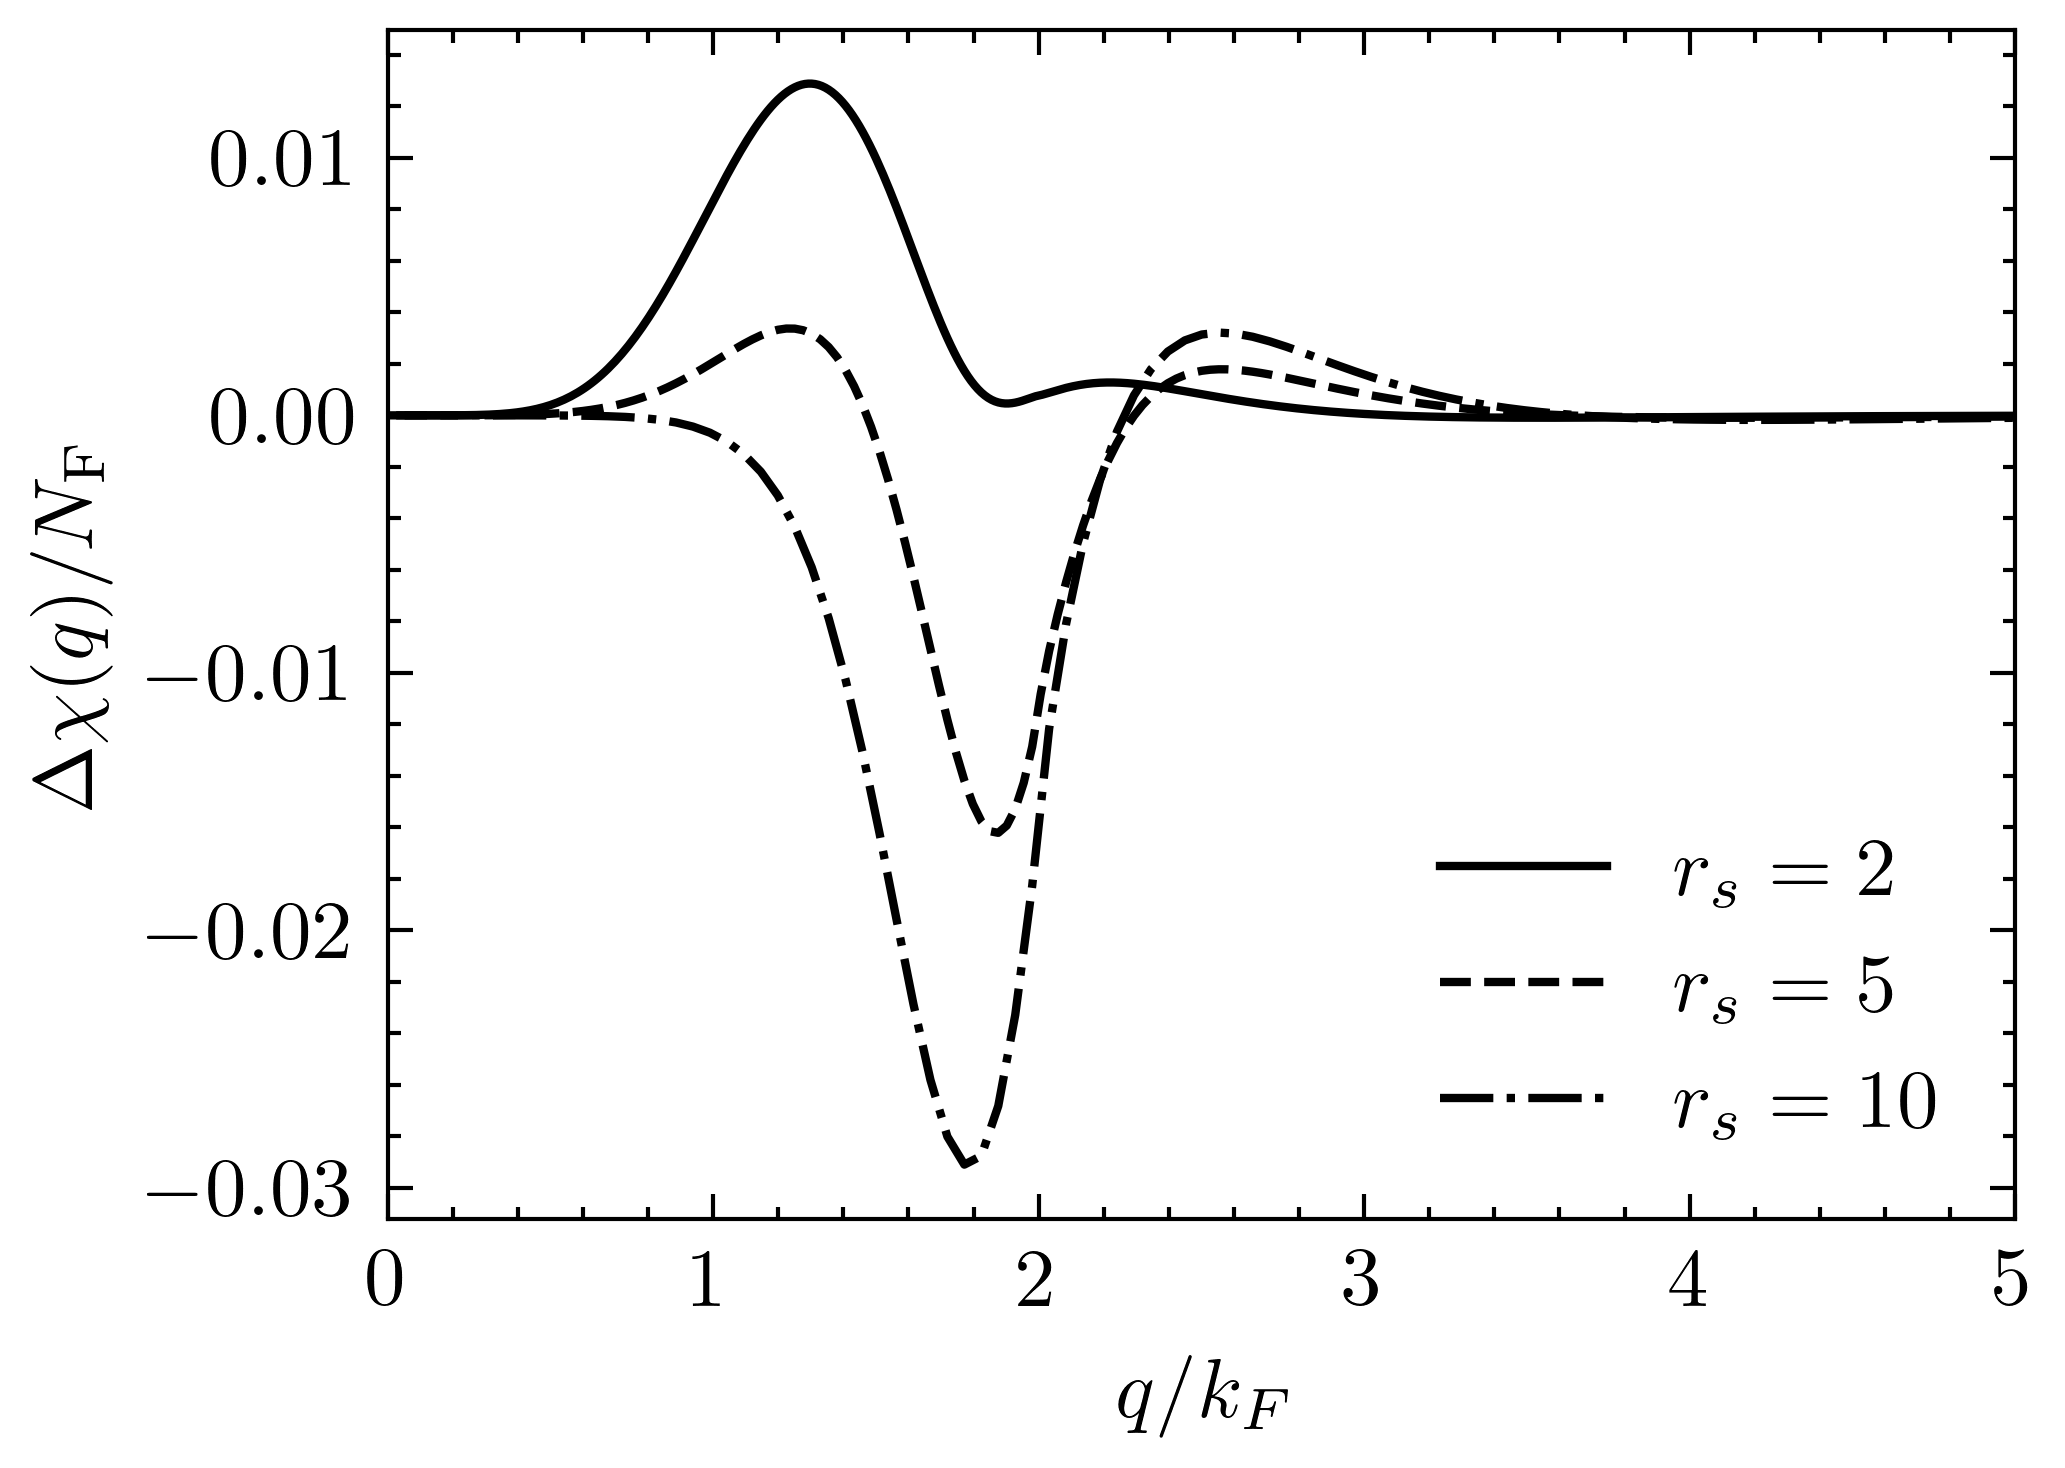
\includegraphics[width=0.5\linewidth]{Figs/qmc_differences.png}
    \caption{Variation between some references in the literature. $\Delta \chi(q)$ corresponds to the  difference of the response functions obtained via \cite{MORONI1995a} and \cite{CORRADINI1998a} for some $r_s$ values.}
    \label{fig:qmc_differences}
\end{figure}
Figure \ref{fig:qmc_differences} shows that variations between these studies are suppressed in the low and high-q limit, which correspond to constraints on the system such as sum rules. In the intermediate q-points, the difference becomes much larger than the statistical error bar especially for $r_s\geq5$. Of course, depending on the application, this difference could be negligible as well as significant.

Even though the real space form is not known, the asymptotic behavior of $\chi(r)$ could be obtained if one calculates the induced density of the electron gas by a delta-like perturbation. Using Lighthill theorem, one can show that this response has the same form as the non-interacting case, with modifications due to interactions affecting only the prefactor, i.e.

\begin{equation}
    \chi(r) \propto -\mathcal{B}\frac{\cos x}{x^3}
\end{equation}

The exact expression of $\mathcal{B}$ and the derivation above is given by \cite{SIMION2005}.

In the same way as before, we have the following low-order moments:

\begin{align}
    C_0 & = 0, \;\;\; C_1 = \frac{3}{8\pi^2},\;\;\; C_2 = \frac{15}{16\pi k_F} + \frac{15f_0}{16\pi^3},\nonumber \\
    C_3 & = \frac{315}{16\,k_F^2\,\pi^4}
    \left(
    f_0^2 k_F^2
    - 4 f_1 k_F^2 \pi
    + 2 f_0 k_F \pi^2
    + \pi^4
    \right)
\end{align}
where $f_0=f_\mathrm{xc}(0)$ and $f_1=f'_\mathrm{xc}(0)$.
\section{Interpolating $\chi(r)$}
We would like to interpolate the interacting response by using as much knowledge from the non-interacting case as we can. We already know that it satisfies certain behaviors, such as $\chi(q) \propto 1/q^2$ for large-$q$ and $\chi(q) \propto/q^2$ low-$q$. Therefore, the intermediate regime constitutes the key region in which interaction effects become important. These points translate to real space the same way. The large-$r$ behavior is exactly known \cite{SIMION2005}, as well as diverging tail as $r\rightarrow 0$ which produces the $1/q^2$ behavior. Thus, we now focus on the intermediate-$r$ region. From Figure \ref{fig:int_vs_nonint} we can already infer that the relevant regime for us would be $k_Fr \simeq [0,6]$.
\begin{figure}
    \centering
    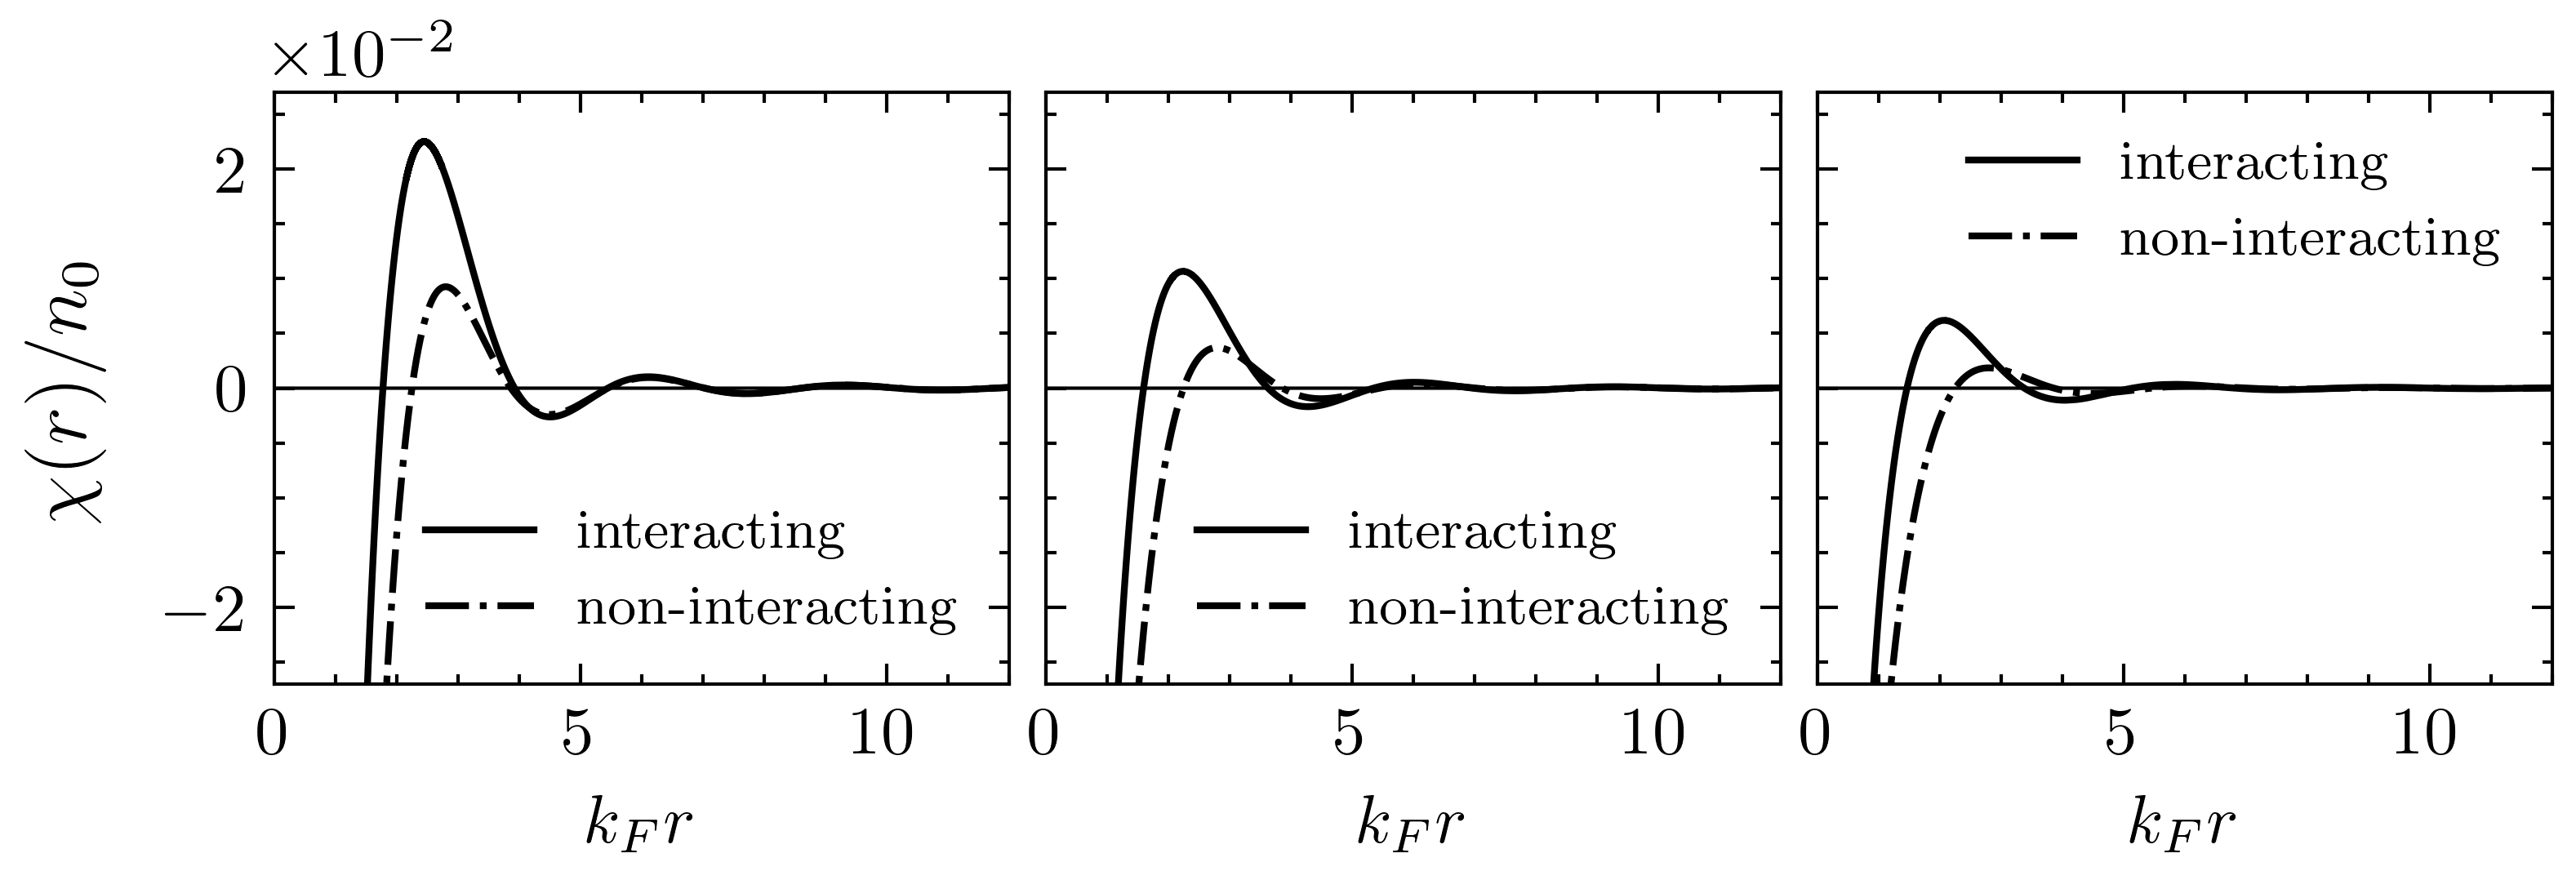
\includegraphics[width=\linewidth]{Figs/int_vs_nonint.png}
    \caption{Static response of the electron gas for $r_s=2,5,10$ (from left to right). The solid line gives the interacting response calculated with Equation \eqref{dyson} with interpolation from \cite{CORRADINI1998a}. The dashdotted line represents the non-interacting response.}
    \label{fig:int_vs_nonint}
\end{figure}

\subsection{The auxiliary function $\mathcal{X}(r)$}
The simplest idea we can try is to subtract the asymptotic part from the full expression of $\chi(r)$, i.e. $\chi(r)+\mathcal{B} \frac{\cos{(2k_F r)}}{(2k_F r)^3}$. However, this does not remove the oscillations fully in the large-$r$ region. Simple inspection shows that there is a residual $\mathcal{B} \frac{\sin{(2k_F r)}}{(2k_F r)^4}$ factor as well. After further removing, we are left with a function that does not oscillate or its oscillations are greatly reduced. It is also interesting to note that the removed piece is nothing but the non-interacting response with its prefactor modified by the interacting response function's asymptotic form, i.e.

$$
    \chi(r) +\mathcal{B} \frac{\cos{(2k_F r)}}{(2k_F r)^3} - \mathcal{B} \frac{\sin{(2k_F r)}}{(2k_F r)^4} = \chi(r) - \frac{\mathcal{B}}{-6\pi n_0 N_F}\chi_0(r)
$$

However, above equation still is not a good candidate to start interpolating since it diverges as $r \rightarrow 0$. One can then try to scale the above equation with $(2k_Fr)^4$ to get rid of the divergence at $r=0$, however that would yield a second term that is $\mathcal{B} (\sin x -x\cos x)$ which blows up asymptotically. Now, we propose the following form that performs much better,

\begin{equation}\label{X_definition}
    \mathcal{X}(r) = \frac{(2k_F r)^4}{r^\gamma}\Bigg(\chi(r) - \frac{\mathcal{B}}{-6\pi n_0 N_F}\chi_0(r)\Bigg)
\end{equation}

With this definition, we see that there are no more divergences, i.e. $\mathcal{X}(r\rightarrow 0) = 0$ and $\mathcal{X}(r\rightarrow \infty) = 0$. This is due to both scaling with $(2k_Fr)^4$, and adding a $1/r^\gamma$ factor which dampens the $\mathcal{B} (\sin x -x\cos x)$ part. For this part, we choose $\gamma=1$, but we will show that other choices can be done and can make optimization more stable. We note that $\mathcal{X}(r)$ decays much faster than $1/r$ which suggests an exponential fitting might be favorable. Lastly, it is straightforward to show that for no interaction, $\mathcal{X}(r)=0$.
\begin{figure}[H]
    \centering
    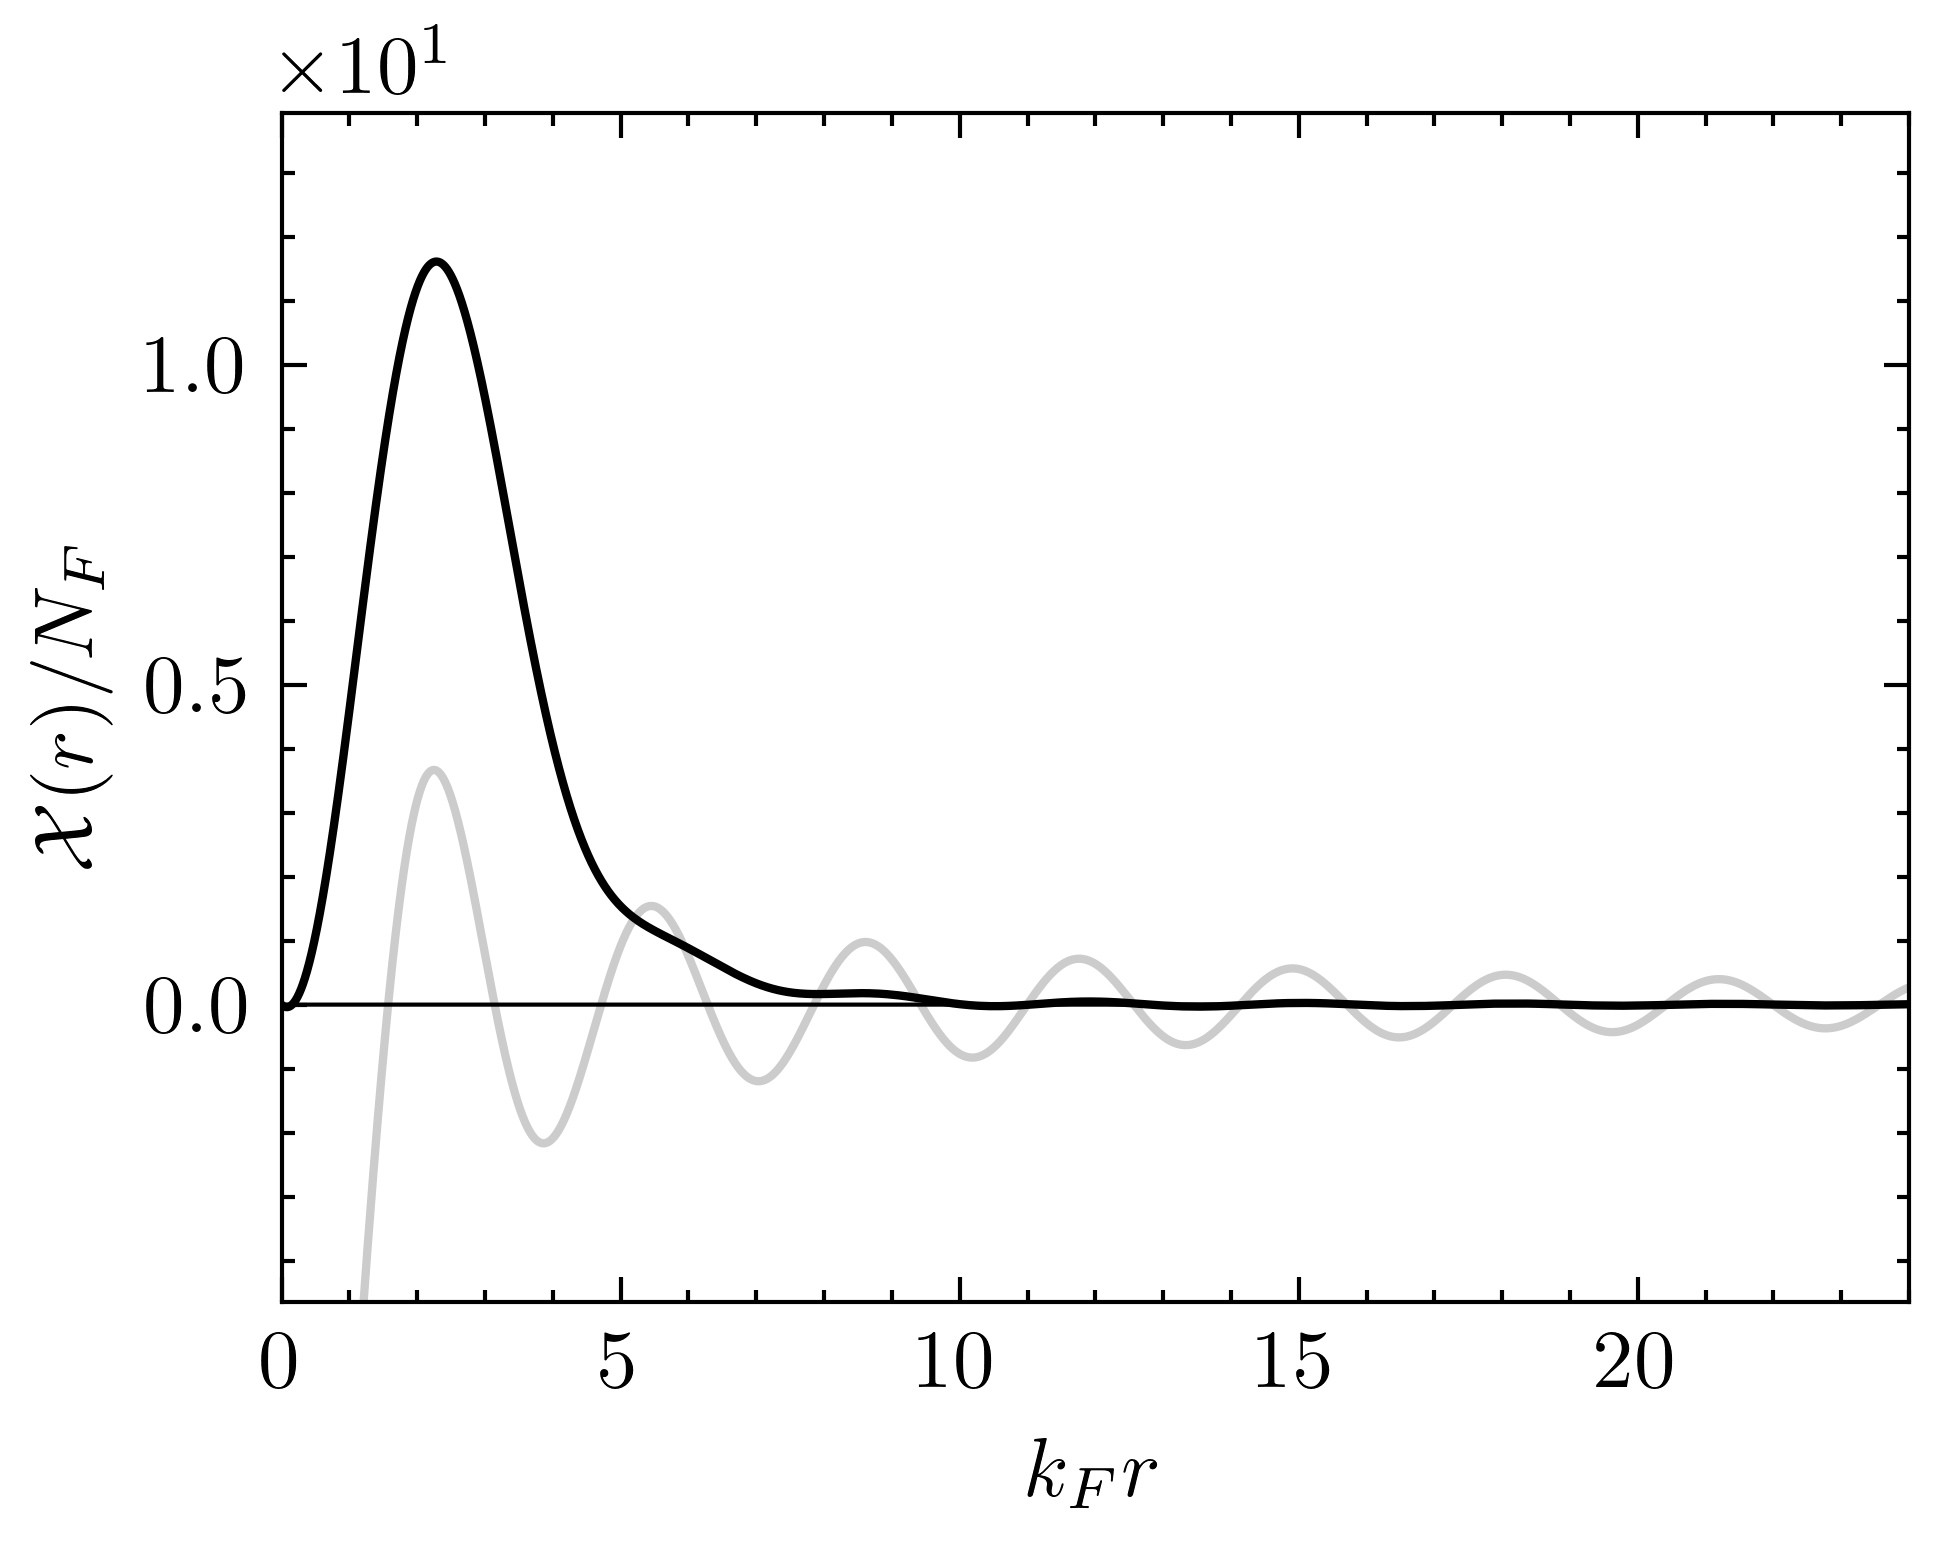
\includegraphics[width=0.48\textwidth]{Figs/X_rs1.png}
    {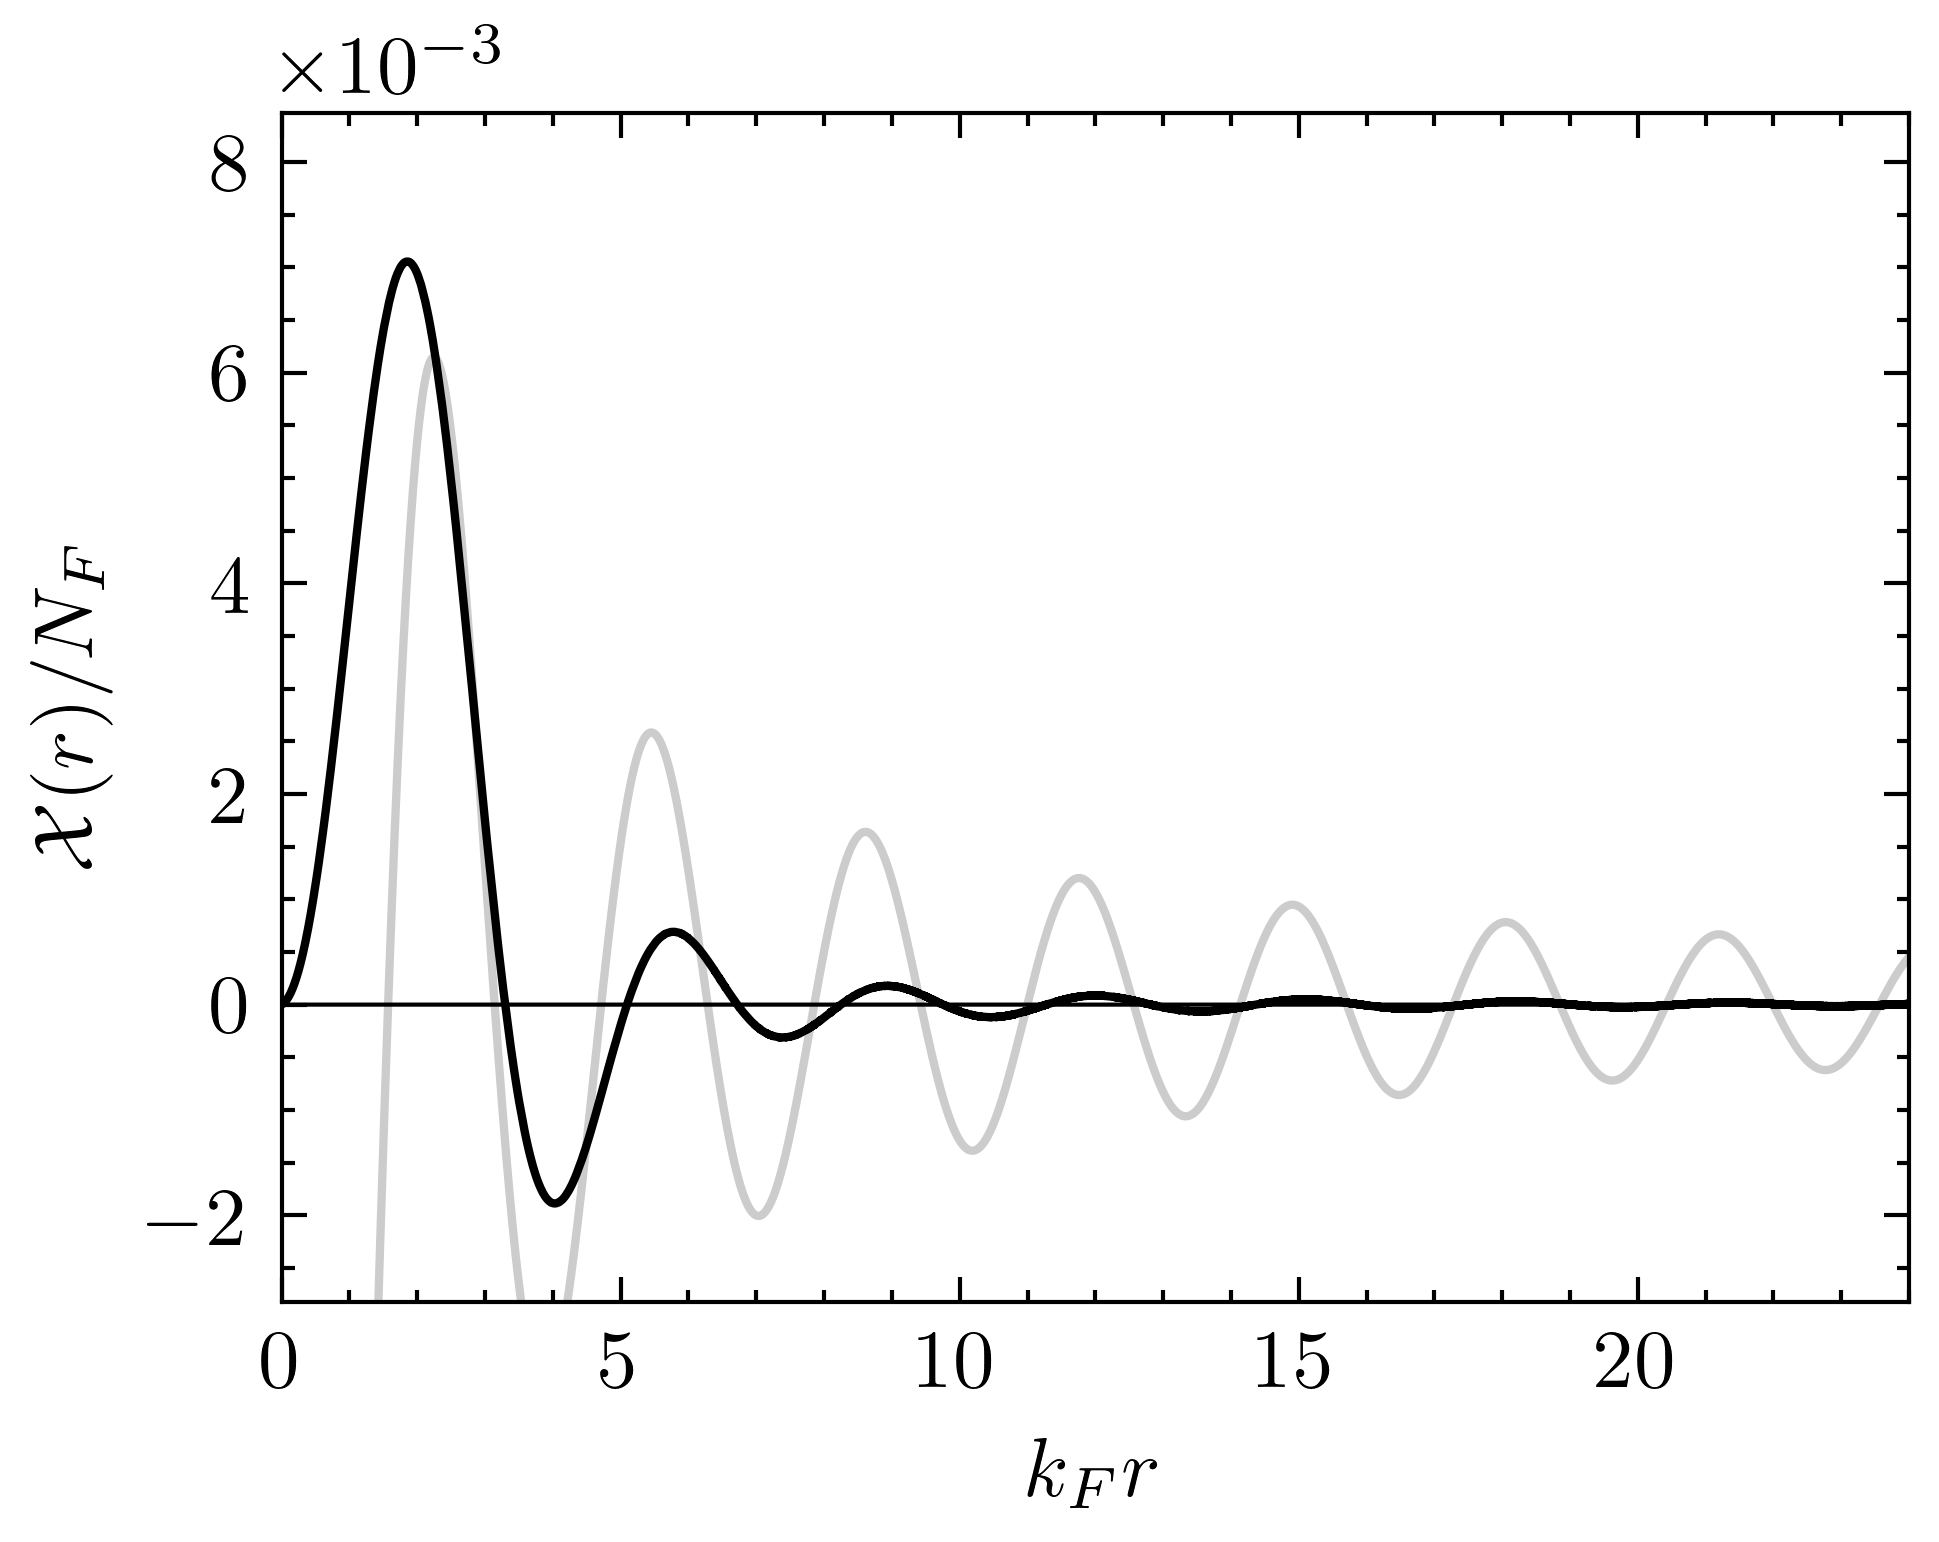
\includegraphics[width=0.48\textwidth]{Figs/X_rs5.png}}
    \caption{\textbf{Left:} Exact $\mathcal{X}(r)$ for $r_s=1$. \textbf{Right:} Exact $\mathcal{X}(r)$ for $r_s=5$. Grey lines correspond to $\mathcal{B}\frac{\sin x}{x}$ (with $x=2k_Fr$) to compare decay rates. $\gamma=2$ for both plots.}
    \label{exact_X}
\end{figure}

\subsubsection{Real-space ansatz}

Figure \ref{exact_X} shows us that $\mathcal{X}(r)$ is a well-behaved, smooth function. To appreciate this function more, we realize that the main peaks around $r=2k_F$ for both $r_s=1$ and $r_s=5$ correspond to the difference between interacting and non-interacting case (see Figure \ref{fig:int_vs_nonint}). From Figure \ref{fig:int_vs_nonint}, we can observe that after this peak, the two response functions quickly converge together. This shows that the main correction comes from the first peak of $\mathcal{X}(r)$, as well as its correct physical limits.

Inspired by above observations, we propose the following ansatz,

\begin{equation}\label{X_ansatz}
    \mathcal{X}(r)=r ^{3-\gamma}\sum_{m=0}^M A_m \cos{(k_mr +\phi_m)}e^{-\alpha_m r},
\end{equation}

with $\gamma=1,2$ and $\alpha_m>0$. We choose this ansatz to have the correct limits (exponential damping for large-$r$ limit and $r^{3-\gamma}$ for $r\rightarrow 0$ limit), as well as the description of the main peak which has an oscillatory behavior. In our optimization, we will focus on finding $\mathcal{X}(r)$ by choosing a small range of $k_Fr$.

\subsubsection{Sum rules}
For a good description of $\mathcal{X}(r)$, we would need to optimize $4M$ parameters which may seem high. To minimize the number of parameters used, we exploit some exact constraints of both $\chi(r)$ and $\chi^0(r)$. Consider the moments of $\chi(r)$,

\begin{align} \label{C_n_derivation}
    C_n & = \int_0^\infty r^{2n+2}\chi(r)dr = \int_0^\infty r^{2n+2} \mathcal{X}(r)\frac{r^\gamma}{(2k_Fr)^4}dr + \frac{\mathcal{B}}{-6\pi n_0N_F}\int_0^\infty r^{2n+2} \chi_0(r)dr \nonumber \\
        & =\frac{1}{(2k_F)^4}\sum_{m=0}^MA_m\int_0^\infty r^{2n+1}\cos{(k_mr +\phi_m)}e^{-\alpha_m r} dr + \frac{\mathcal{B}}{-6\pi n_0N_F}C_n^0
\end{align}
defining the following and recalling its solution,
\begin{align} \label{I_n_m}
    I^m_n\equiv I_n(k_m,\phi_m,\alpha_m) & =\int_0^\infty r^{2n+1}\cos{(k_mr +\phi_m)}e^{-\alpha_m r} dr \nonumber \\
                                         & =(2n+1)!\;\Re\!\left[ \frac{e^{i\phi_m}}{(\alpha_m - ik_m)^{\,2n+2}}
        \right].
\end{align}

We know have the following sum rule for $\mathcal{X}(r)$. Combining Equations \eqref{C_n_derivation} and \eqref{I_n_m},

\begin{equation}
    \sum_{m=0}^MA_mI^m_n= 16k_F^4\Big(C_n -\frac{\mathcal{B}}{-6\pi n_0N_F} C^0_n\Big) \equiv C^\mathcal{X}_n.
\end{equation}
This gives us \(N\) constraints that we can apply to \(4M\) degrees of freedom. However, these constraints are linear only in the amplitudes \(\{A_m\}\);
the remaining parameters \(\{k_m,\alpha_m,\phi_m\}\) enter the moments through
the nonlinear dependence of \(I_n^m\). As a consequence, the sum rules can be
used at this stage to fix the amplitudes uniquely for any prescribed choice of
the nonlinear parameters, while determining the latter requires solving a
coupled nonlinear problem.

For a given set of moment indices \(\{n_j\}_{j=1}^N\), it is convenient to
introduce the moment vector \(\mathbf{C}^{\mathcal X}\) and the amplitude vector
\(\mathbf A\),
\[
    \mathbf{C}^{\mathcal X} =
    \begin{pmatrix}
        C^{\mathcal X}_{n_1} \\
        C^{\mathcal X}_{n_2} \\
        \vdots               \\
        C^{\mathcal X}_{n_N}
    \end{pmatrix},
    \qquad
    \mathbf A =
    \begin{pmatrix}
        A_0    \\
        A_1    \\
        \vdots \\
        A_M
    \end{pmatrix},
\]
together with the moment matrix \(\mathbf I\) with elements
\[
    \bigl[\mathbf I\bigr]_{j m} \equiv I_{n_j}^m(k_m,\phi_m,\alpha_m).
\]
The sum rules then take the compact matrix form
\begin{equation}
    \mathbf I\,\mathbf A = \mathbf C^{\mathcal X}.
    \label{eq:matrix_sum_rules}
\end{equation}
For fixed \(\{k_m,\alpha_m,\phi_m\}\), Eq.~\eqref{eq:matrix_sum_rules} constitutes
a linear system for the amplitudes \(\{A_m\}\), which can be solved exactly when \(N=M+1\), or in a least-squares sense when \(N>M+1\). In the remainder of this
section, we therefore focus on the determination of the amplitudes from the sum
rules, and defer the discussion of how the nonlinear parameters are fixed to a
later section.

Increasing the number of enforced moments \(N\) would in principle improve the representation. However, each additional mode introduces three new nonlinear parameters \((k_m,\alpha_m,\phi_m)\) in addition to the linear amplitude \(A_m\), so that increasing \(N\) must be accompanied by an increase in the number of modes \(M\). This rapidly enlarges the nonlinear parameter space and limits the practical number of constraints that can be imposed. We therefore adopt the minimal nontrivial choice \(M=1\) (two modes) and enforce \(N=2\) moment constraints, which fixes the amplitudes uniquely while keeping the number of nonlinear parameters manageable.



\subsection{Normalized difference $\Delta{\chi}(r)$}
In this section, we study a different form which again relates to the difference between the interacting and non-interacting case. We simply look at the normalized difference between $\chi$ $\chi_0$, i.e.
\begin{equation}\label{delta_chi_definition}
    \Delta{\chi}(r) = \frac{\chi(r)-\chi_0(r)}{-6\pi n_0 N_F}
\end{equation}

We want to try this form, because as it turns out, $\Delta \chi$ behaves much less oscillatory than $\mathcal{X}$, although having the same real-space range.

\subsubsection{Real-space ansatz}
This can be thought of an instance of $\mathcal{X}$ from equation \eqref{X_ansatz}, i.e. $\mathcal{X}(\gamma=3)$.
\begin{equation}\label{delta_chi_ansatz}
    \Delta{\chi}(r)=\sum_{m=0}^M A_m \cos{(k_mr +\phi_m)}e^{-\alpha_m r}
\end{equation}

\subsubsection{Sum Rules}
At this point, the sum rules are straightforward and follows the same procedure as the previous section.
\begin{align} \label{delta_C_n_derivation}
    C_n & = \int_0^\infty r^{2n+2}\chi(r)dr = \int_0^\infty r^{2n+2}\chi_0(r)dr - 6\pi n_0 N_F  \int_0^\infty r^{2n+2}\Delta{\chi}(r)dr \nonumber \\
        & = C_n^0 -6\pi n_0 N_F \sum_{m=0}^M A_m J_n^m
\end{align}
defining the following and recalling its solution,


\begin{equation} \label{J_n_m}
    J^m_n\equiv J_n(k_m,\phi_m,\alpha_m) =\int_0^\infty r^{2n+2}\cos{(k_mr +\phi_m)}e^{-\alpha_m r} dr = I^m_{n+1}
\end{equation}

We know have the following sum rule for $\Delta{\chi}(r)$. Combining Equations \eqref{delta_C_n_derivation} and \eqref{J_n_m}, we obtain the new sum rule as the normalized difference of individual moments, i.e.

\begin{equation}
    \sum_{m=0}^MA_mJ^m_n= \frac{C_n - C_n^0}{-6\pi n_0 N_F} \equiv \Delta C_n.
\end{equation}

The sum rules then take the compact matrix form,
\begin{equation}
    \mathbf J\,\mathbf A = \mathbf{\Delta C}.
    \label{eq:matrix_sum_rules2}
\end{equation}

\subsubsection{Nonlinear moment constraints}

While the sum rules discussed above allow us to determine the amplitudes
$\{A_m\}$ for any prescribed set of nonlinear parameters
$\{k_m,\alpha_m,\phi_m\}$, the latter remain unconstrained at this stage.
Additional information can be extracted by considering multiple moments
simultaneously and exploiting the explicit trigonometric structure of the
integrals $I_n^m$.

Using the closed-form expression \eqref{I_n_m}, each moment can be written as
\begin{equation}
    I_n^m
    =
    \Lambda_n^m
    \Big[
        C_n^m \cos\phi_m
        -
        D_n^m \sin\phi_m
        \Big],
\end{equation}
where
\[
    \Lambda_n^m = \frac{(2n+1)!}{(\alpha_m^2+k_m^2)^{n+1}},
\]
and where $C_n^m$ and $D_n^m$ are known polynomials in $(k_m,\alpha_m)$ whose
explicit form follows from expanding $(\alpha_m-ik_m)^{-(2n+2)}$.
The precise expressions are not required for the present discussion; it is
sufficient to note that they depend only on $(k_m,\alpha_m)$ and are independent
of the phases $\phi_m$.

For a given set of moment indices $\{n_j\}_{j=1}^N$, the sum rules
\eqref{eq:matrix_sum_rules} can then be written explicitly as
\begin{equation}
    \sum_{m=0}^M
    A_m \Lambda_{n_j}^m
    \bigl[
        C_{n_j}^m \cos\phi_m
        -
        D_{n_j}^m \sin\phi_m
        \bigr]
    =
    C_{n_j}^{\mathcal X},
    \qquad j=1,\dots,N.
\end{equation}

For the minimal choice $M=2$ (two modes) and $N=2$ moments, this yields a system
of four coupled equations involving the four trigonometric quantities
$\{\cos\phi_0,\sin\phi_0,\cos\phi_1,\sin\phi_1\}$. Introducing the vector
\[
    \mathbf v =
    \begin{pmatrix}
        \cos\phi_0 \\
        \sin\phi_0 \\
        \cos\phi_1 \\
        \sin\phi_1
    \end{pmatrix},
\]
the constraints can be cast into the compact matrix form
\begin{equation}
    \mathbf M(k_m,\alpha_m)\,\mathbf v = \mathbf b,
    \label{eq:nonlinear_matrix}
\end{equation}
where the $4\times4$ matrix $\mathbf M$ depends parametrically on the decay
rates $\{\alpha_m\}$ and wave vectors $\{k_m\}$ through the coefficients
$\Lambda_n^m$, $C_n^m$, and $D_n^m$, and where the right-hand side $\mathbf b$
contains the corresponding four moment combinations $C_n^{\mathcal X}$.

Equation~\eqref{eq:nonlinear_matrix} highlights the fundamentally nonlinear
character of the problem: although it is linear in the trigonometric functions
of the phases, the coefficients themselves depend nonlinearly on
$(k_m,\alpha_m)$. As a result, the determination of the nonlinear parameters
requires solving a coupled nonlinear system, in contrast to the purely linear
problem encountered for the amplitudes.

Despite this, one can try to at least use~\eqref{eq:nonlinear_matrix} to fix the phases, $\phi_m$. However, even though we now use more moments to constrain the system, the results (not shown here but can be checked in \cite{GUNES}) get worse. This may be because linearizing the phase allows different moments to constrain
$\cos\phi_m$ and $\sin\phi_m$ independently, even though they should originate
from a single complex mode. As higher moments emphasize different length scales,
these constraints can become incompatible for a minimal ansatz, whereas the
nonlinear formulation preserves their coupling. In the following section, we will only focus on the previous two methods and not~\eqref{eq:nonlinear_matrix}.



\section{Results}
\FloatBarrier
The results are obtained via the following procedure:
\begin{itemize}
    \item Initialize the six nonlinear parameters
          $\{\alpha_m,k_m,\phi_m\}_{m=0,1}$.
    \item Fix the amplitudes $\{A_m\}$ exactly using the moment sum rules using~\eqref{eq:matrix_sum_rules} for $\mathcal{X}$-interpolation and~\eqref{eq:matrix_sum_rules2} for $\Delta{\chi}$-interpolation.
    \item Optimize the nonlinear parameters by minimizing a least-squares
          residual between the reconstructed quantity ($\mathcal{X}$ or $\Delta{\chi}$) and the exact reference data in real space over a finite range of $k_F r$.
    \item Propagate the solution smoothly as a function of $r_s$ using the previous
          optimum as the initial condition.
    \item If needed, do an inverse sweep starting from the last $r_s$ parameters.
\end{itemize}
At the end of the procedure, we obtain a dictionary of parameters as a function of $r_s$. At this point, it is straightforward to obtain the response function, one must use equation~\eqref{X_definition} for $\mathcal{X}$-interpolation and equation~\eqref{delta_chi_definition} for $\Delta{\chi}$-interpolation. In the following plots, I present the real space response function as well as the reciprocal space version since our interpolation must satisfy the low and high-$q$ limit. I also show the normalized errors which gives us an idea of how successful the interpolation is.


\begin{figure}[h!]
    \centering
    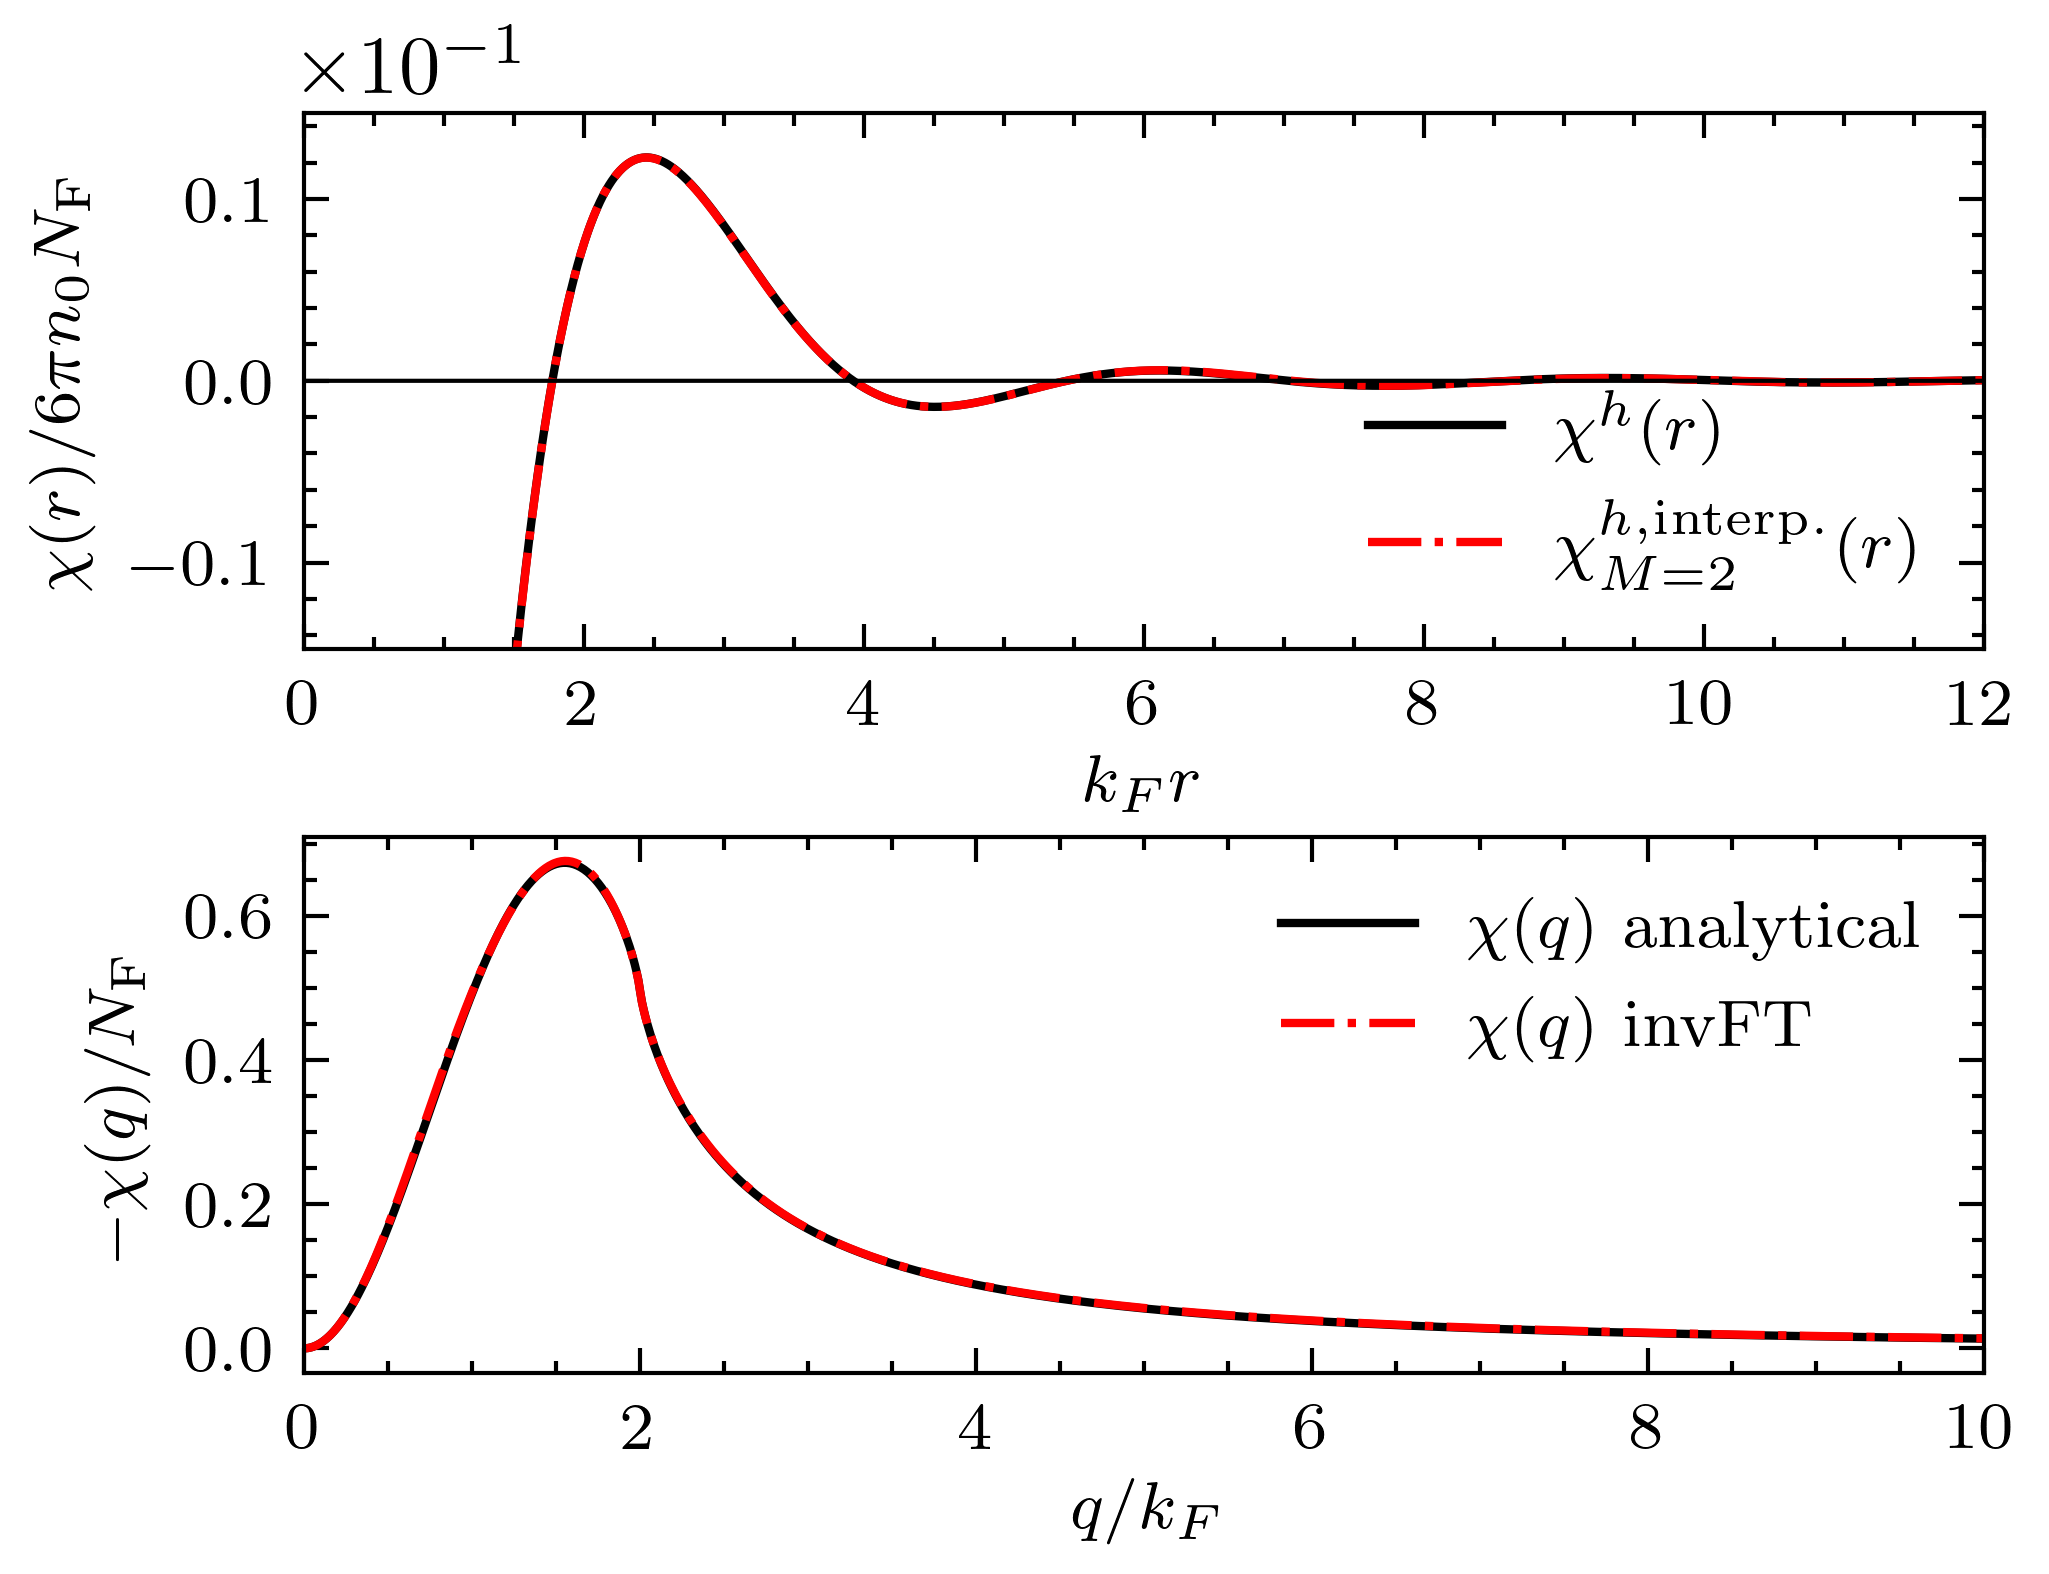
\includegraphics[width=0.46\textwidth]{Figs/X-rs2-error0.png}
    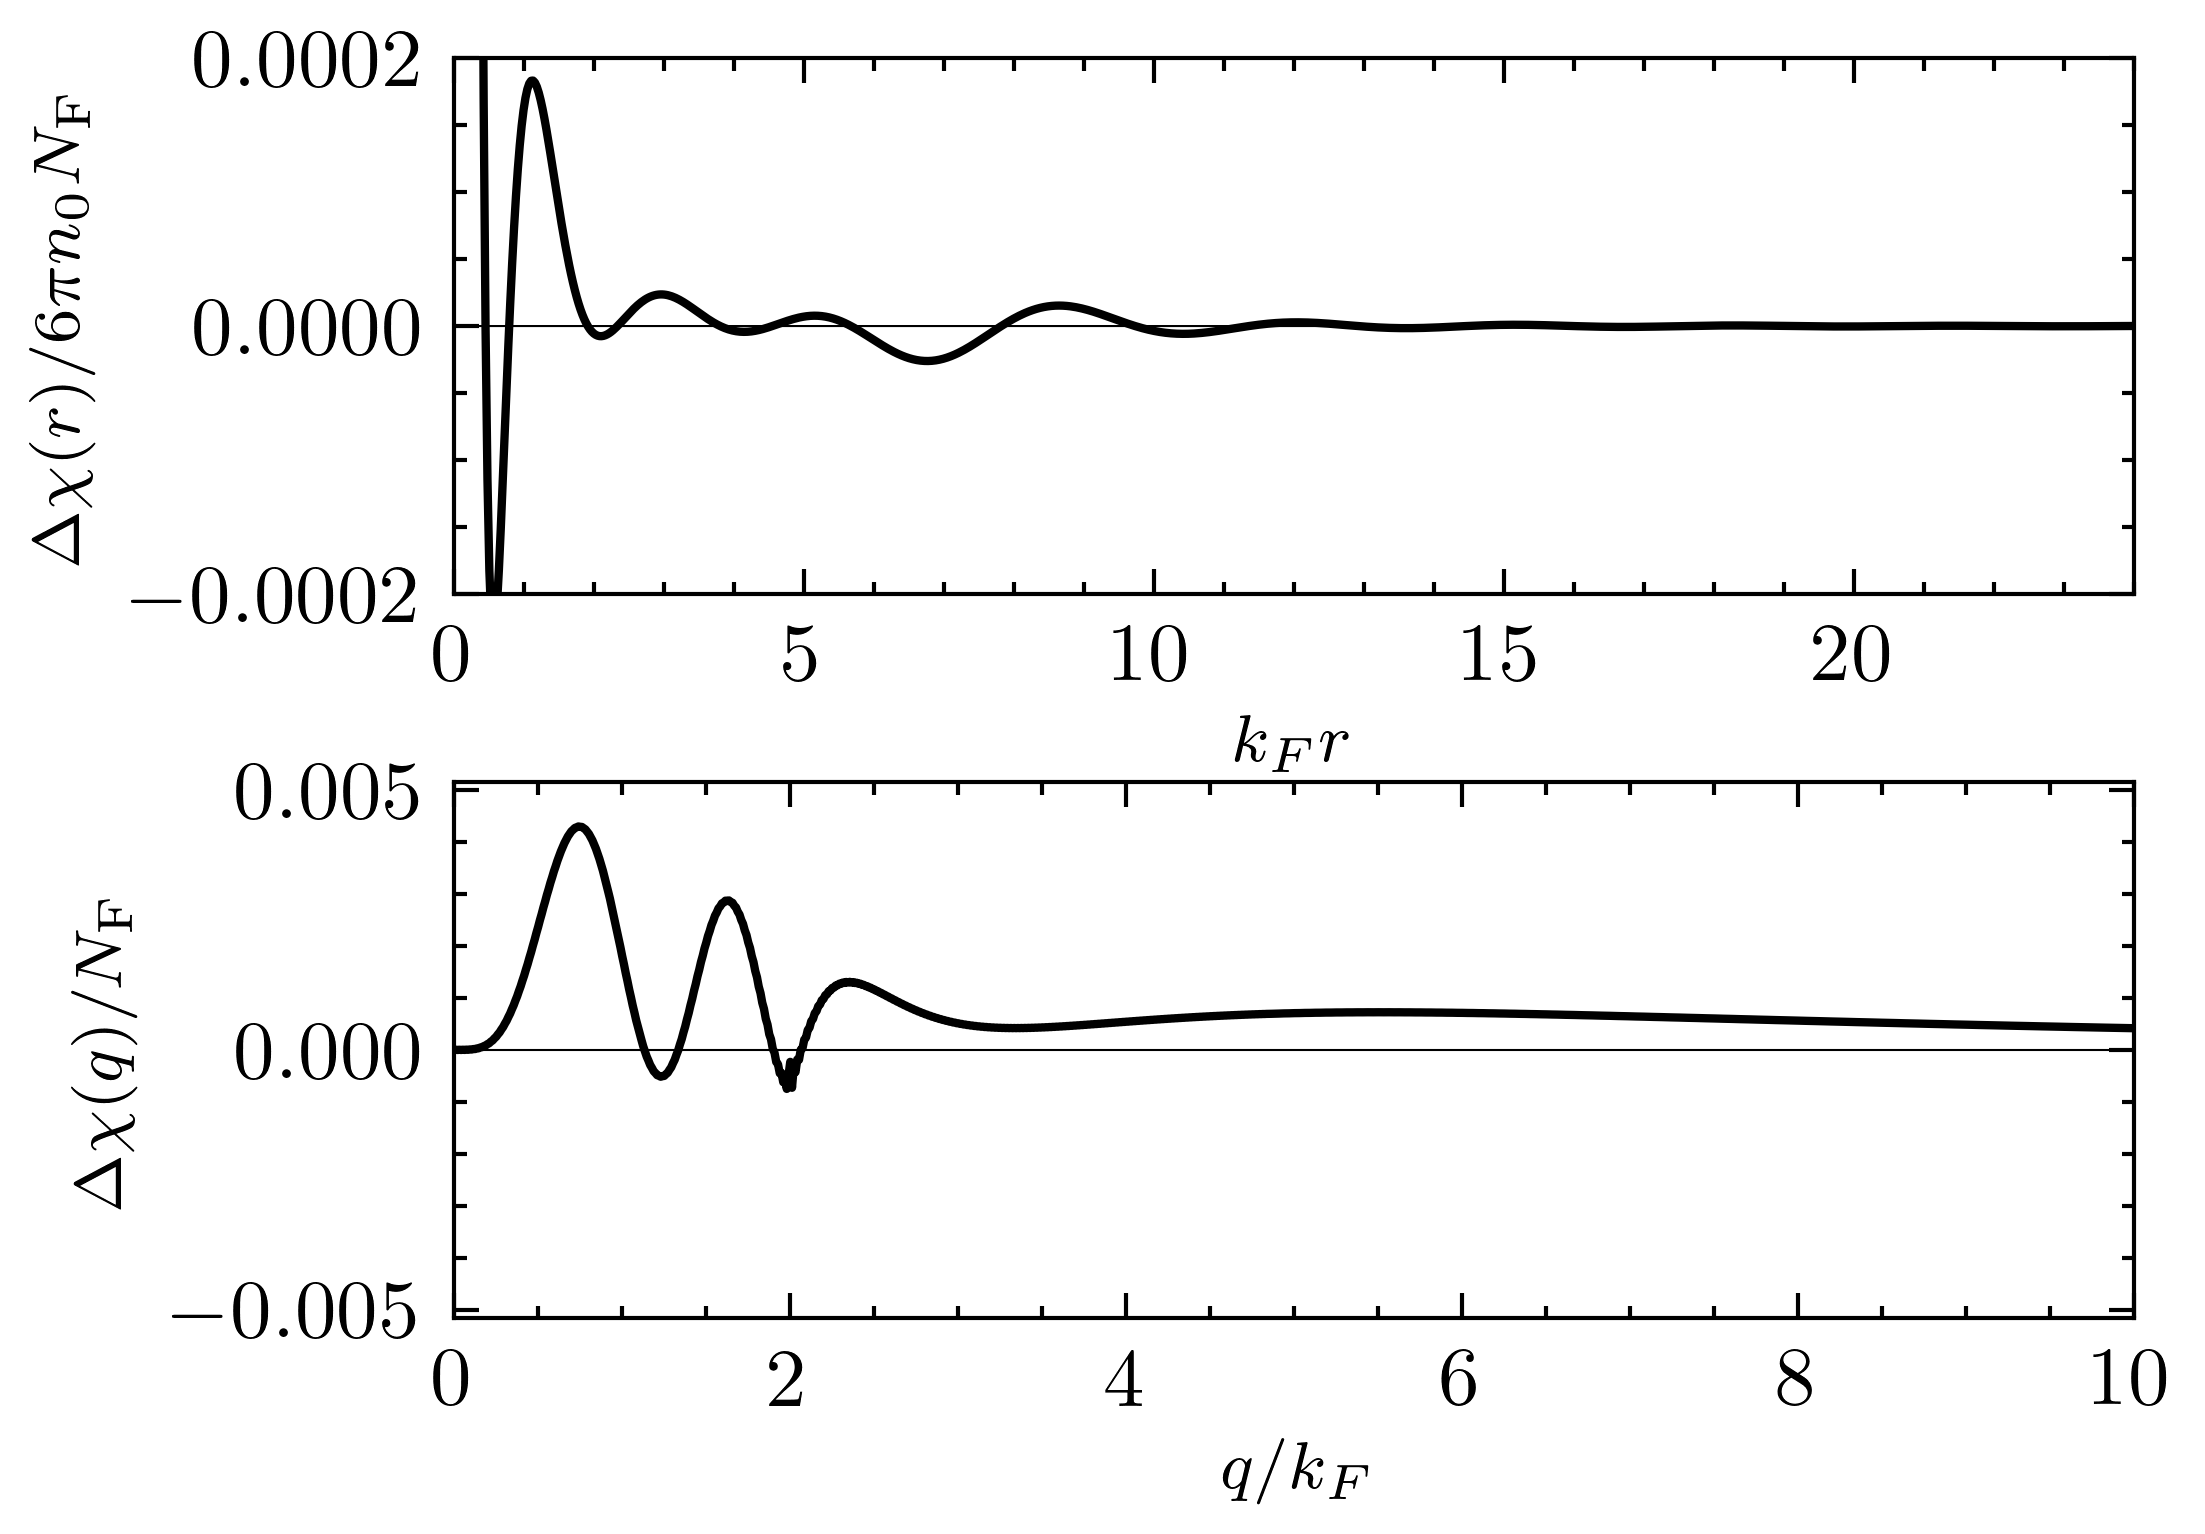
\includegraphics[width=0.49\textwidth]{Figs/X-rs2-error1.png}
    \caption{{\textbf{Left:}} Static response calculated by $\mathcal{X}$-interpolation (in red) in comparison with the exact result (in black) for $r_s = 2$. {\textbf{Right:}} Normalized absolute error in static response calculated by $\mathcal{X}$-interpolation. Upper panels show the real space quantities, and lower panel shows the reciprocal space quantities.}
    \label{fig:X-rs2}
\end{figure}

\begin{figure}
    \centering
    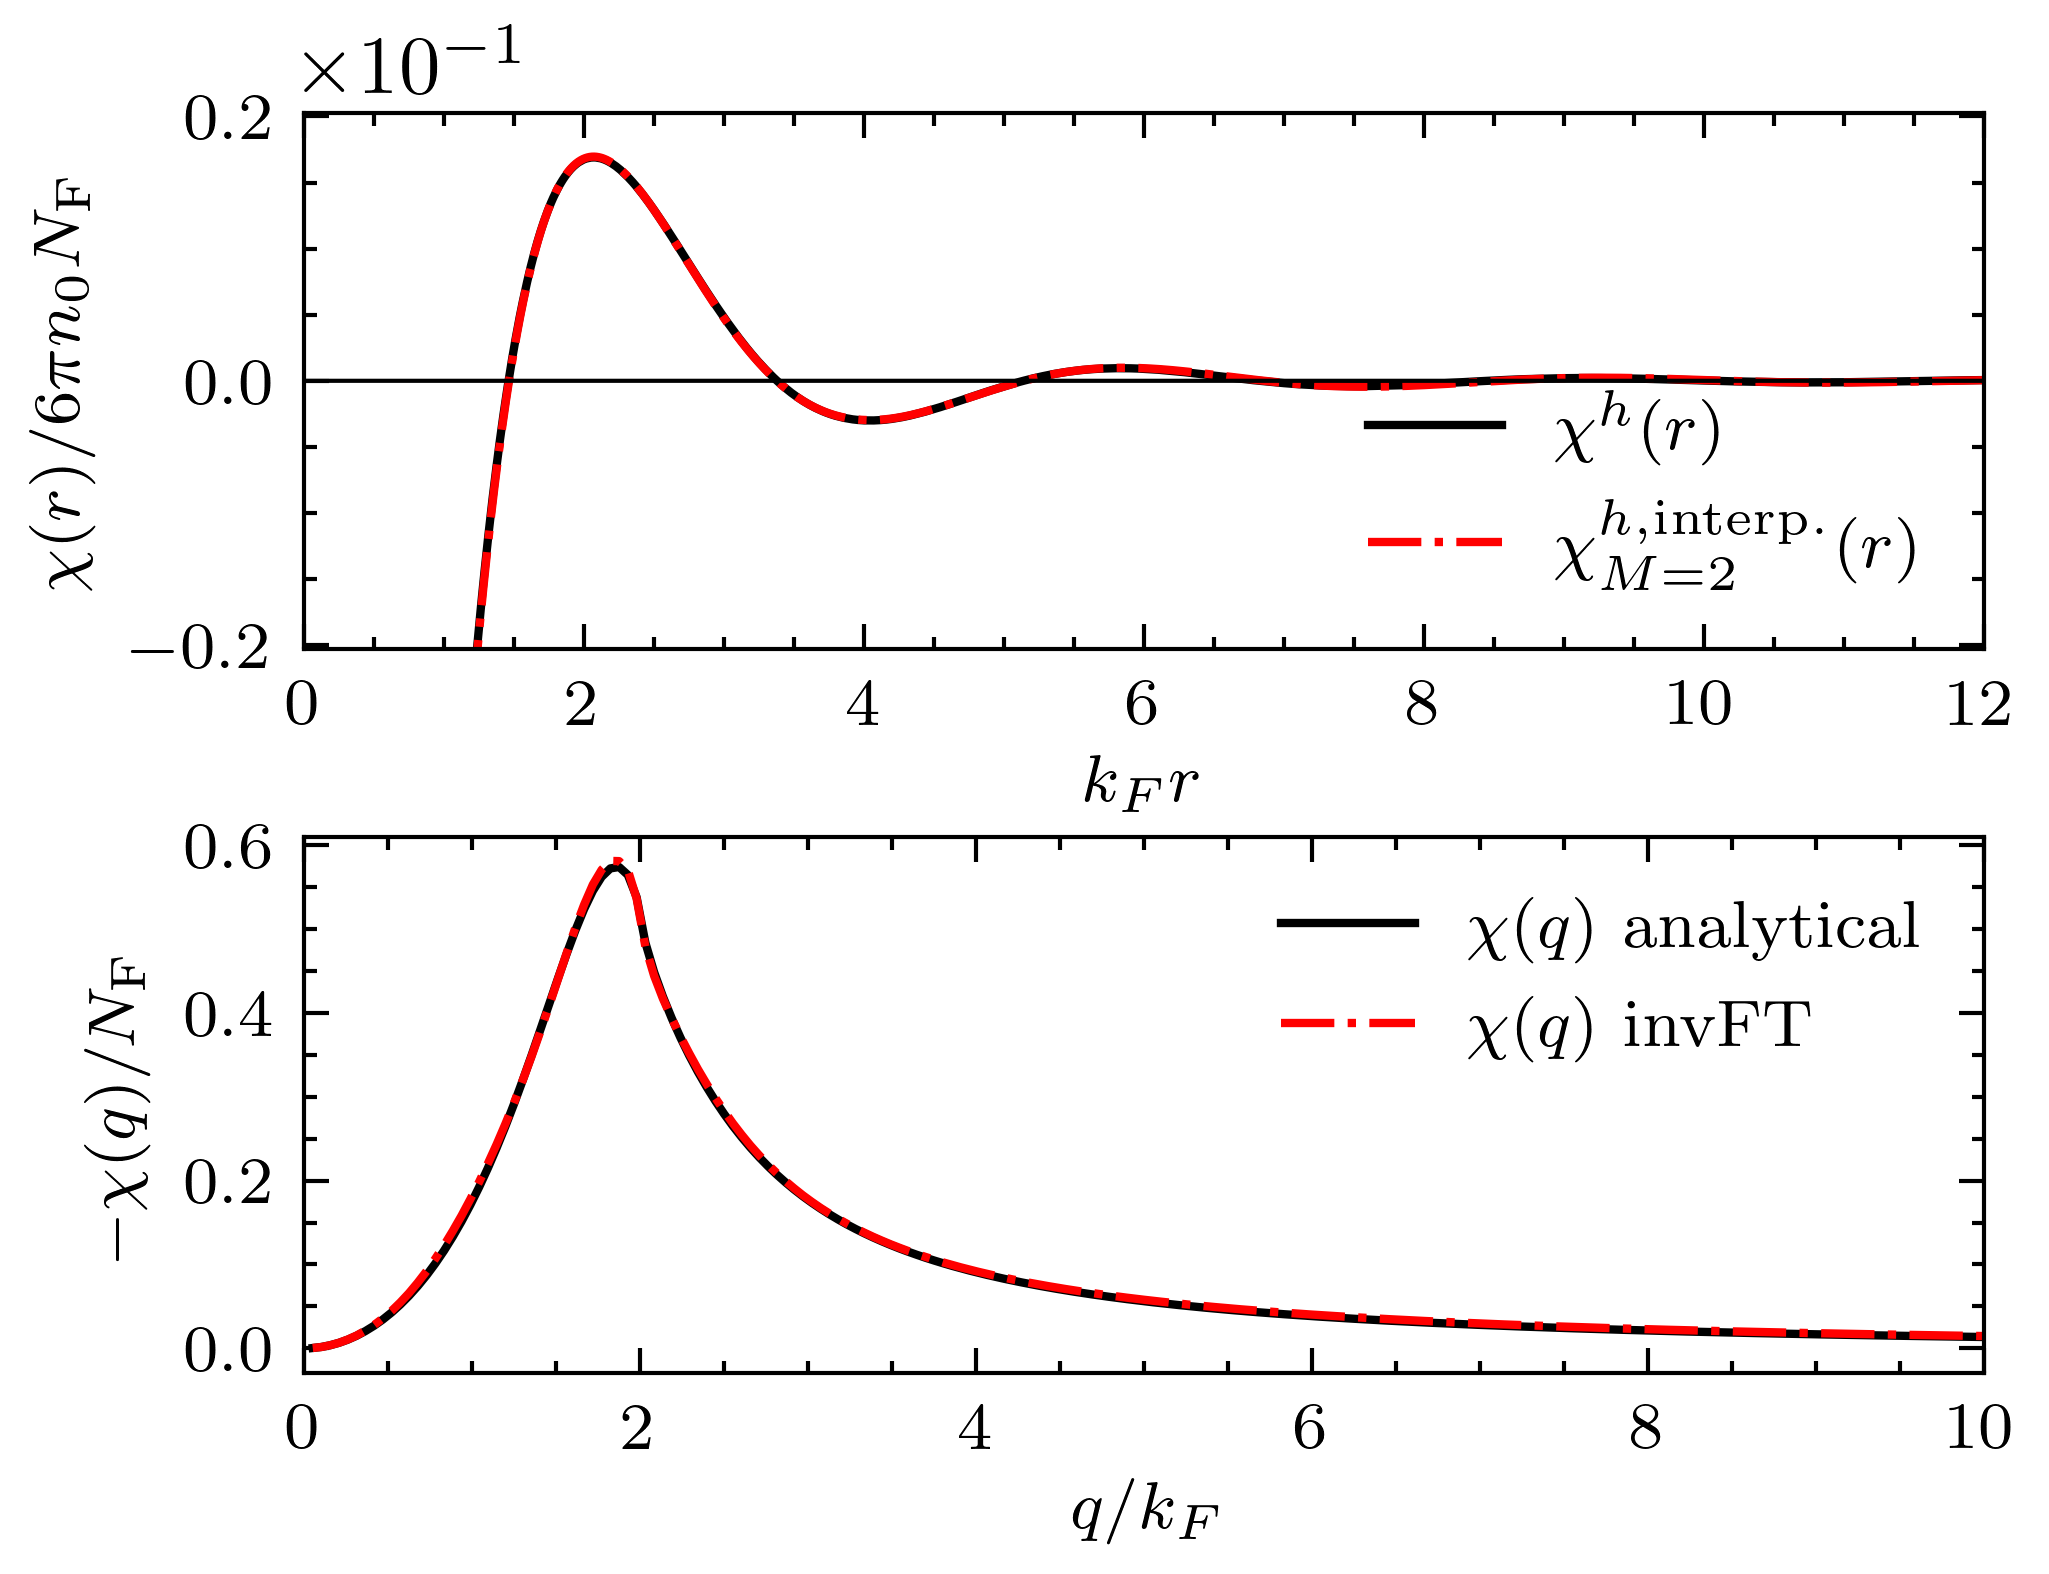
\includegraphics[width=0.46\textwidth]{Figs/X-rs10-error0.png}
    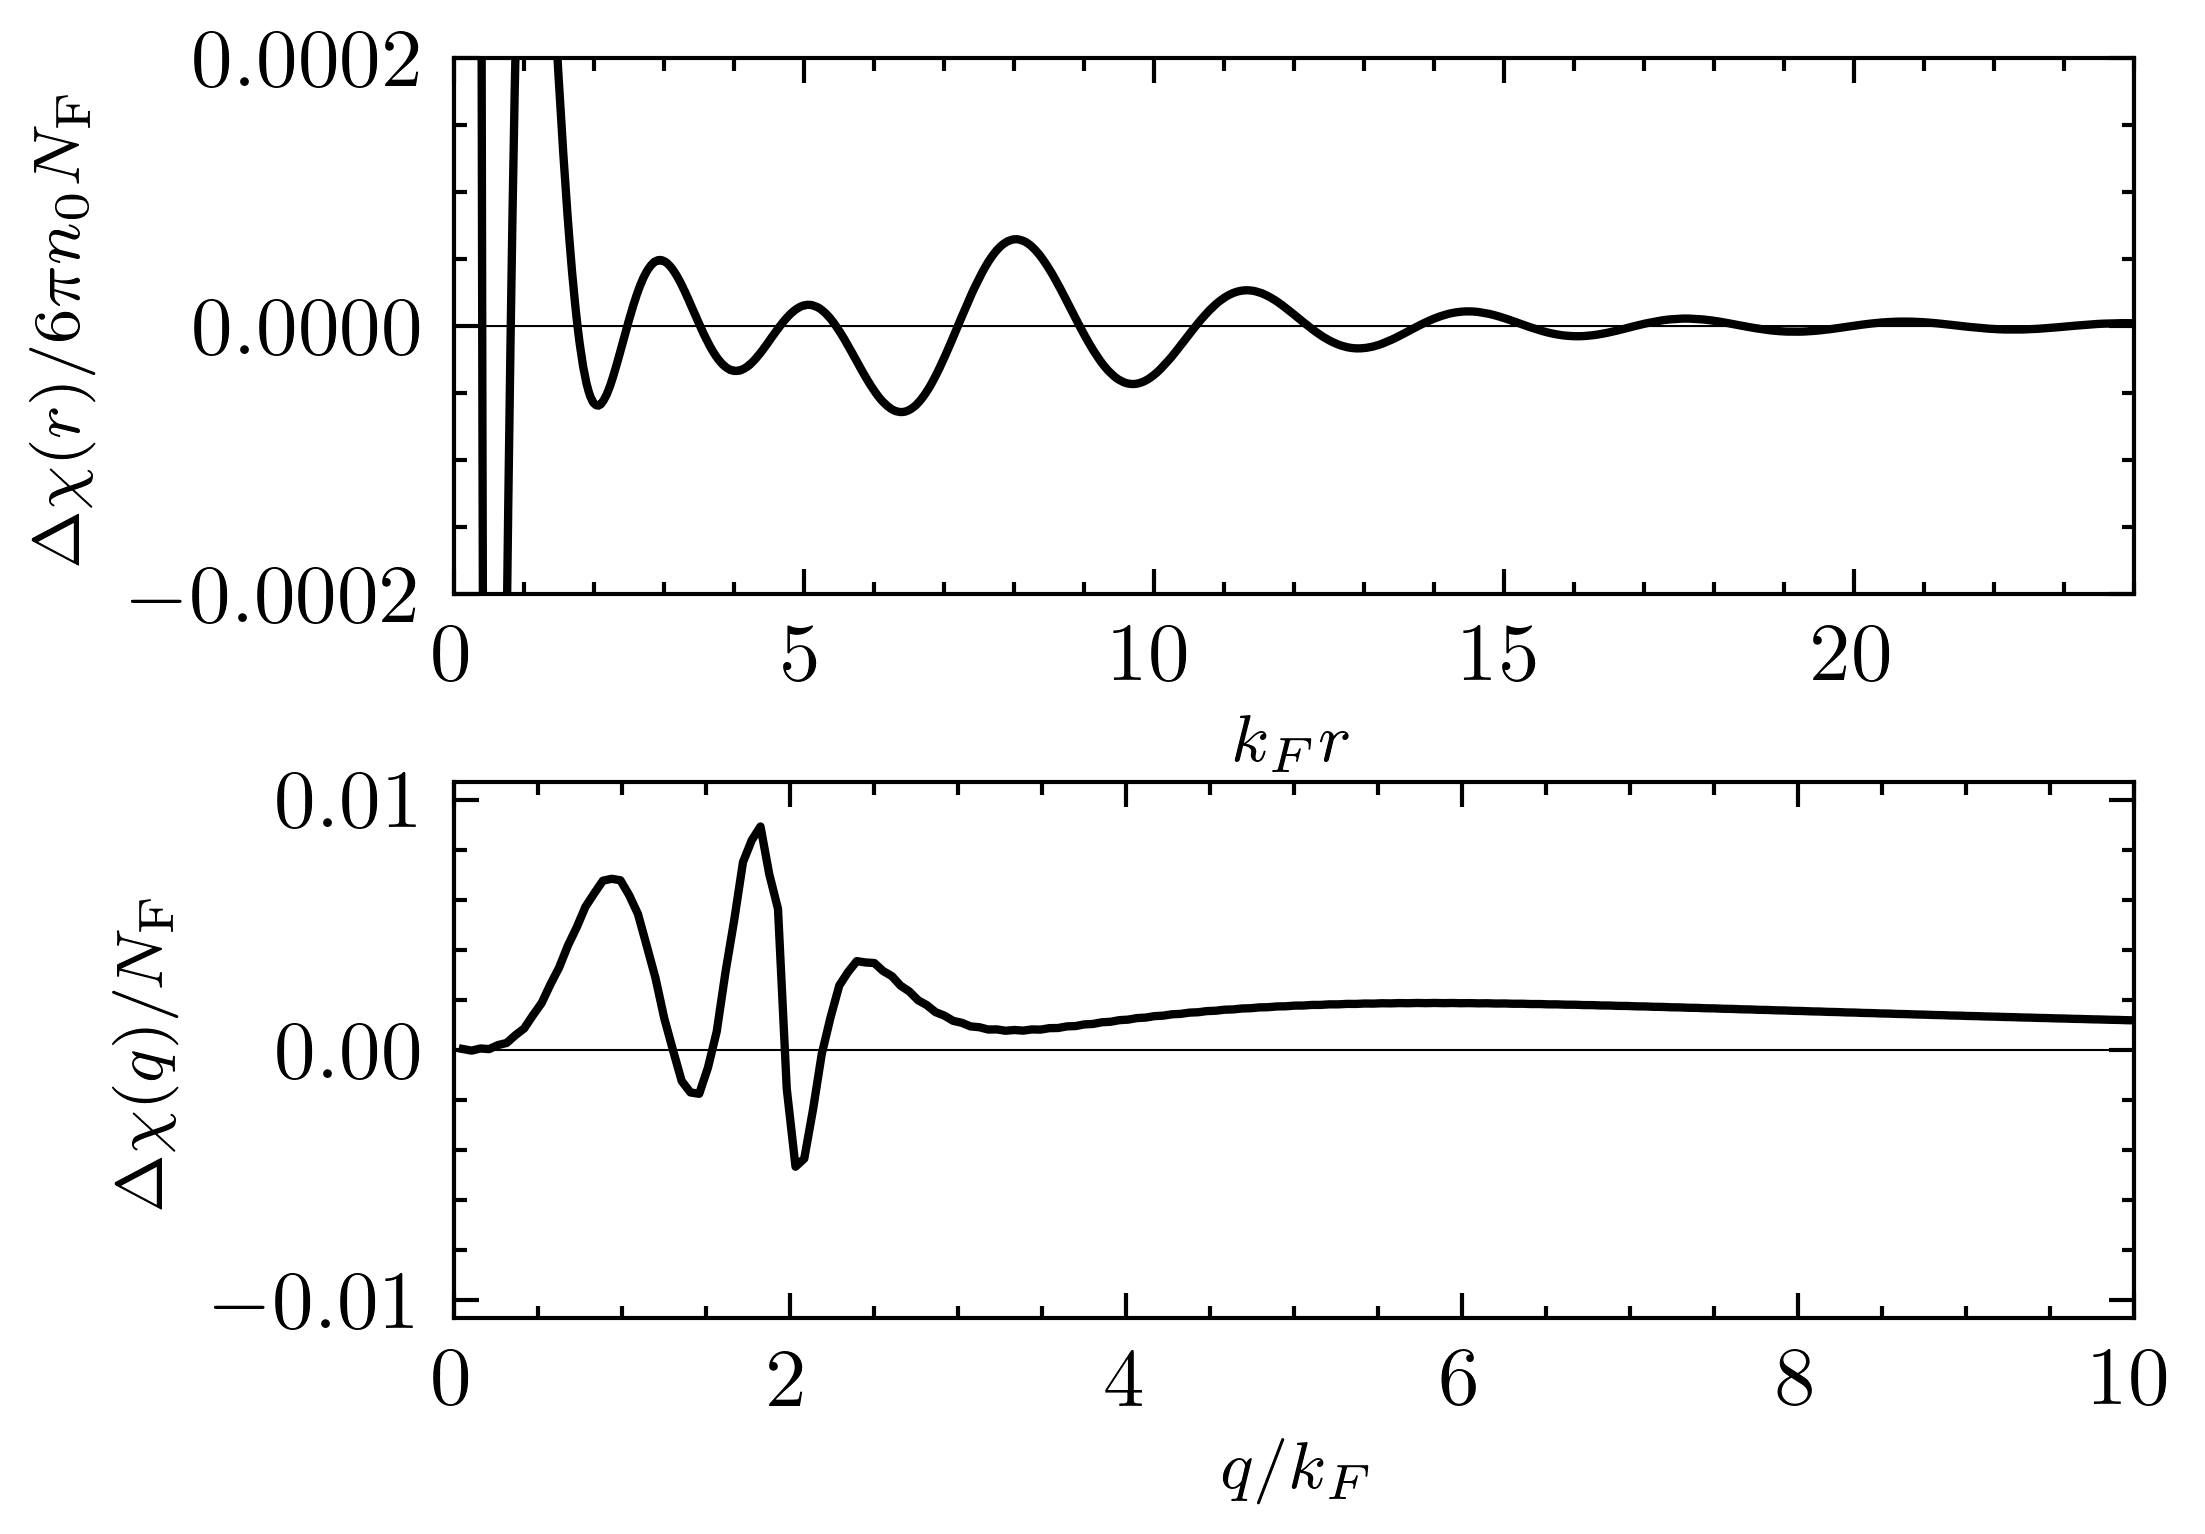
\includegraphics[width=0.49\textwidth]{Figs/X-rs10-error1.png}
    \caption{{\textbf{Left:}} Static response calculated by $\mathcal{X}$-interpolation (in red) in comparison with the exact result (in black) for $r_s = 10$. {\textbf{Right:}} Normalized absolute error in static response calculated by $\mathcal{X}$-interpolation. Upper panels show the real space quantities, and lower panel shows the reciprocal space quantities.}
    \label{fig:X-rs10}
\end{figure}

Results given in Figures \ref{fig:X-rs2} and \ref{fig:X-rs10} are obtained with $\gamma=2$. As we can see, the interpolation results are indistinguishable to the eye for both real-space and reciprocal-space. However, the error analysis shows that the high-$q$ error (which correspond to interpolating the low-$r$) does not decay smoothly until very large $q/k_F$. The reason for this is due to the definition of $\mathcal{X}$. From equation~\eqref{X_ansatz}, we see that due to the $r^{3-\gamma}$ factor $\mathcal{X}(r\rightarrow0)=0$ which implies the interacting and non-interacting response functions become equivalent. In reality, this difference is nonzero and converges to a finite value. This is the main cause of the relatively large error around $k_Fr=0$ in Figures \ref{fig:X-rs2} and \ref{fig:X-rs10} (top right panels).




\begin{figure}
    \centering
    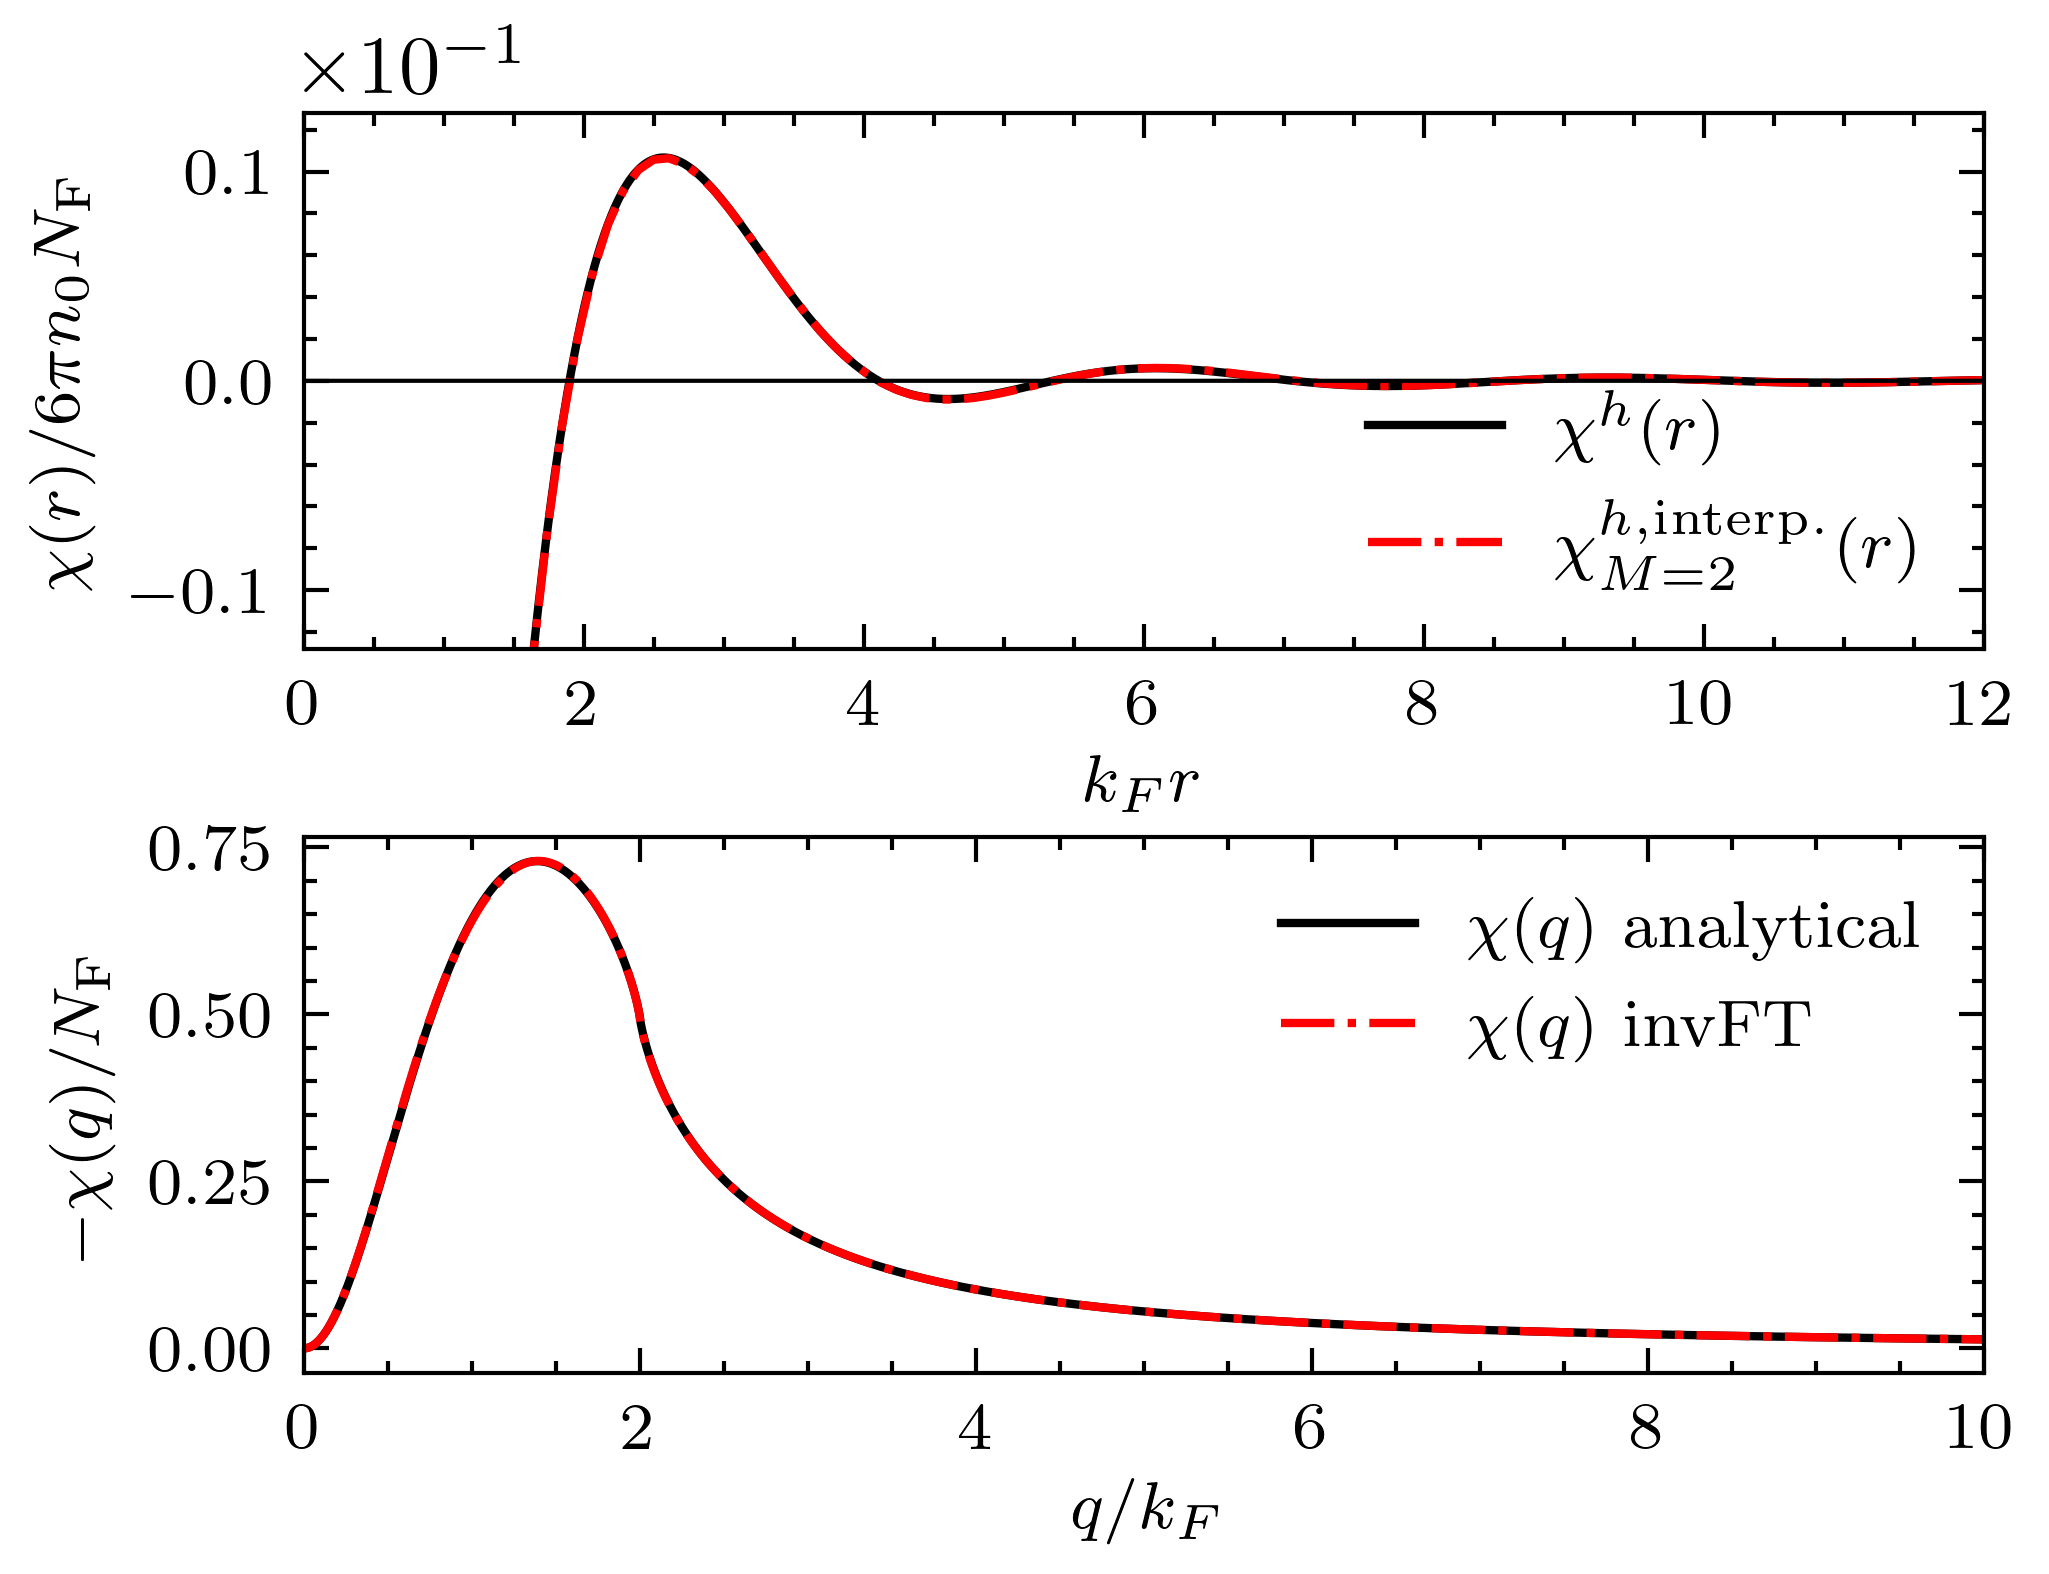
\includegraphics[width=0.46\textwidth]{Figs/delta_chi-rs1-error0.png}
    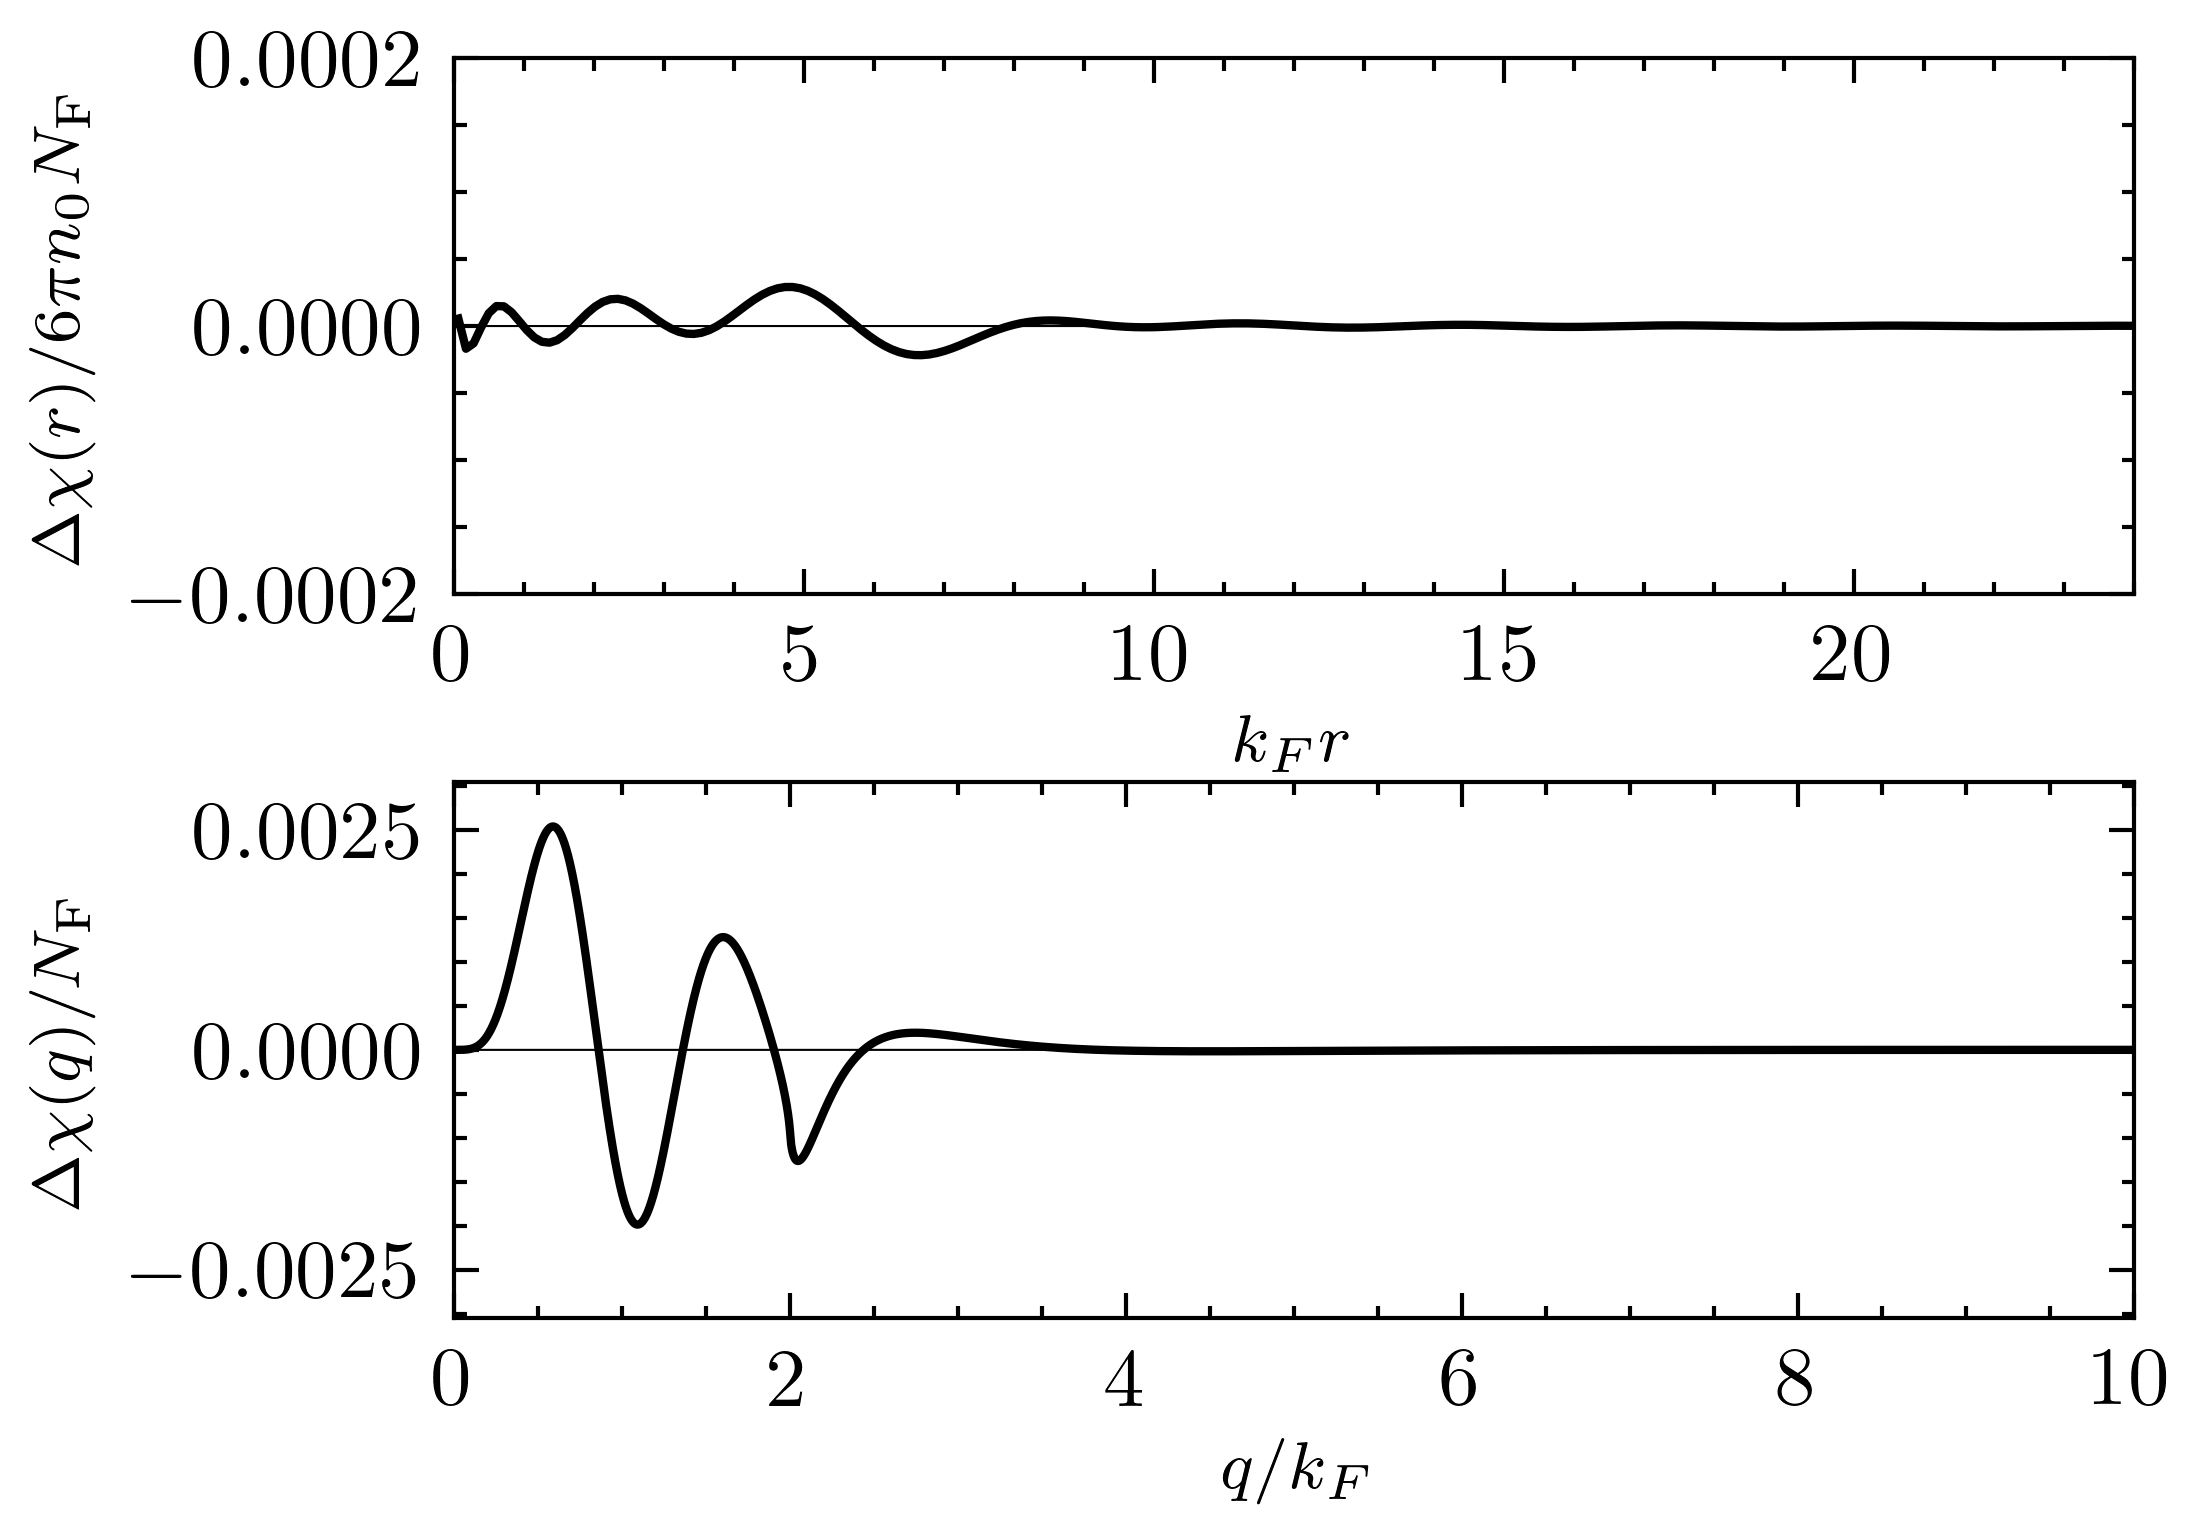
\includegraphics[width=0.49\textwidth]{Figs/delta_chi-rs1-error1.png}
    \caption{{\textbf{Left:}} Static response calculated by $\Delta{\chi}$-interpolation (in red) in comparison with the exact result (in black) for $r_s = 1$. {\textbf{Right:}} Normalized absolute error in static response calculated by $\Delta{\chi}$-interpolation. Upper panels show the real space quantities, and lower panel shows the reciprocal space quantities.}
    \label{fig:delta_chi-rs1}
\end{figure}

\begin{figure}
    \centering
    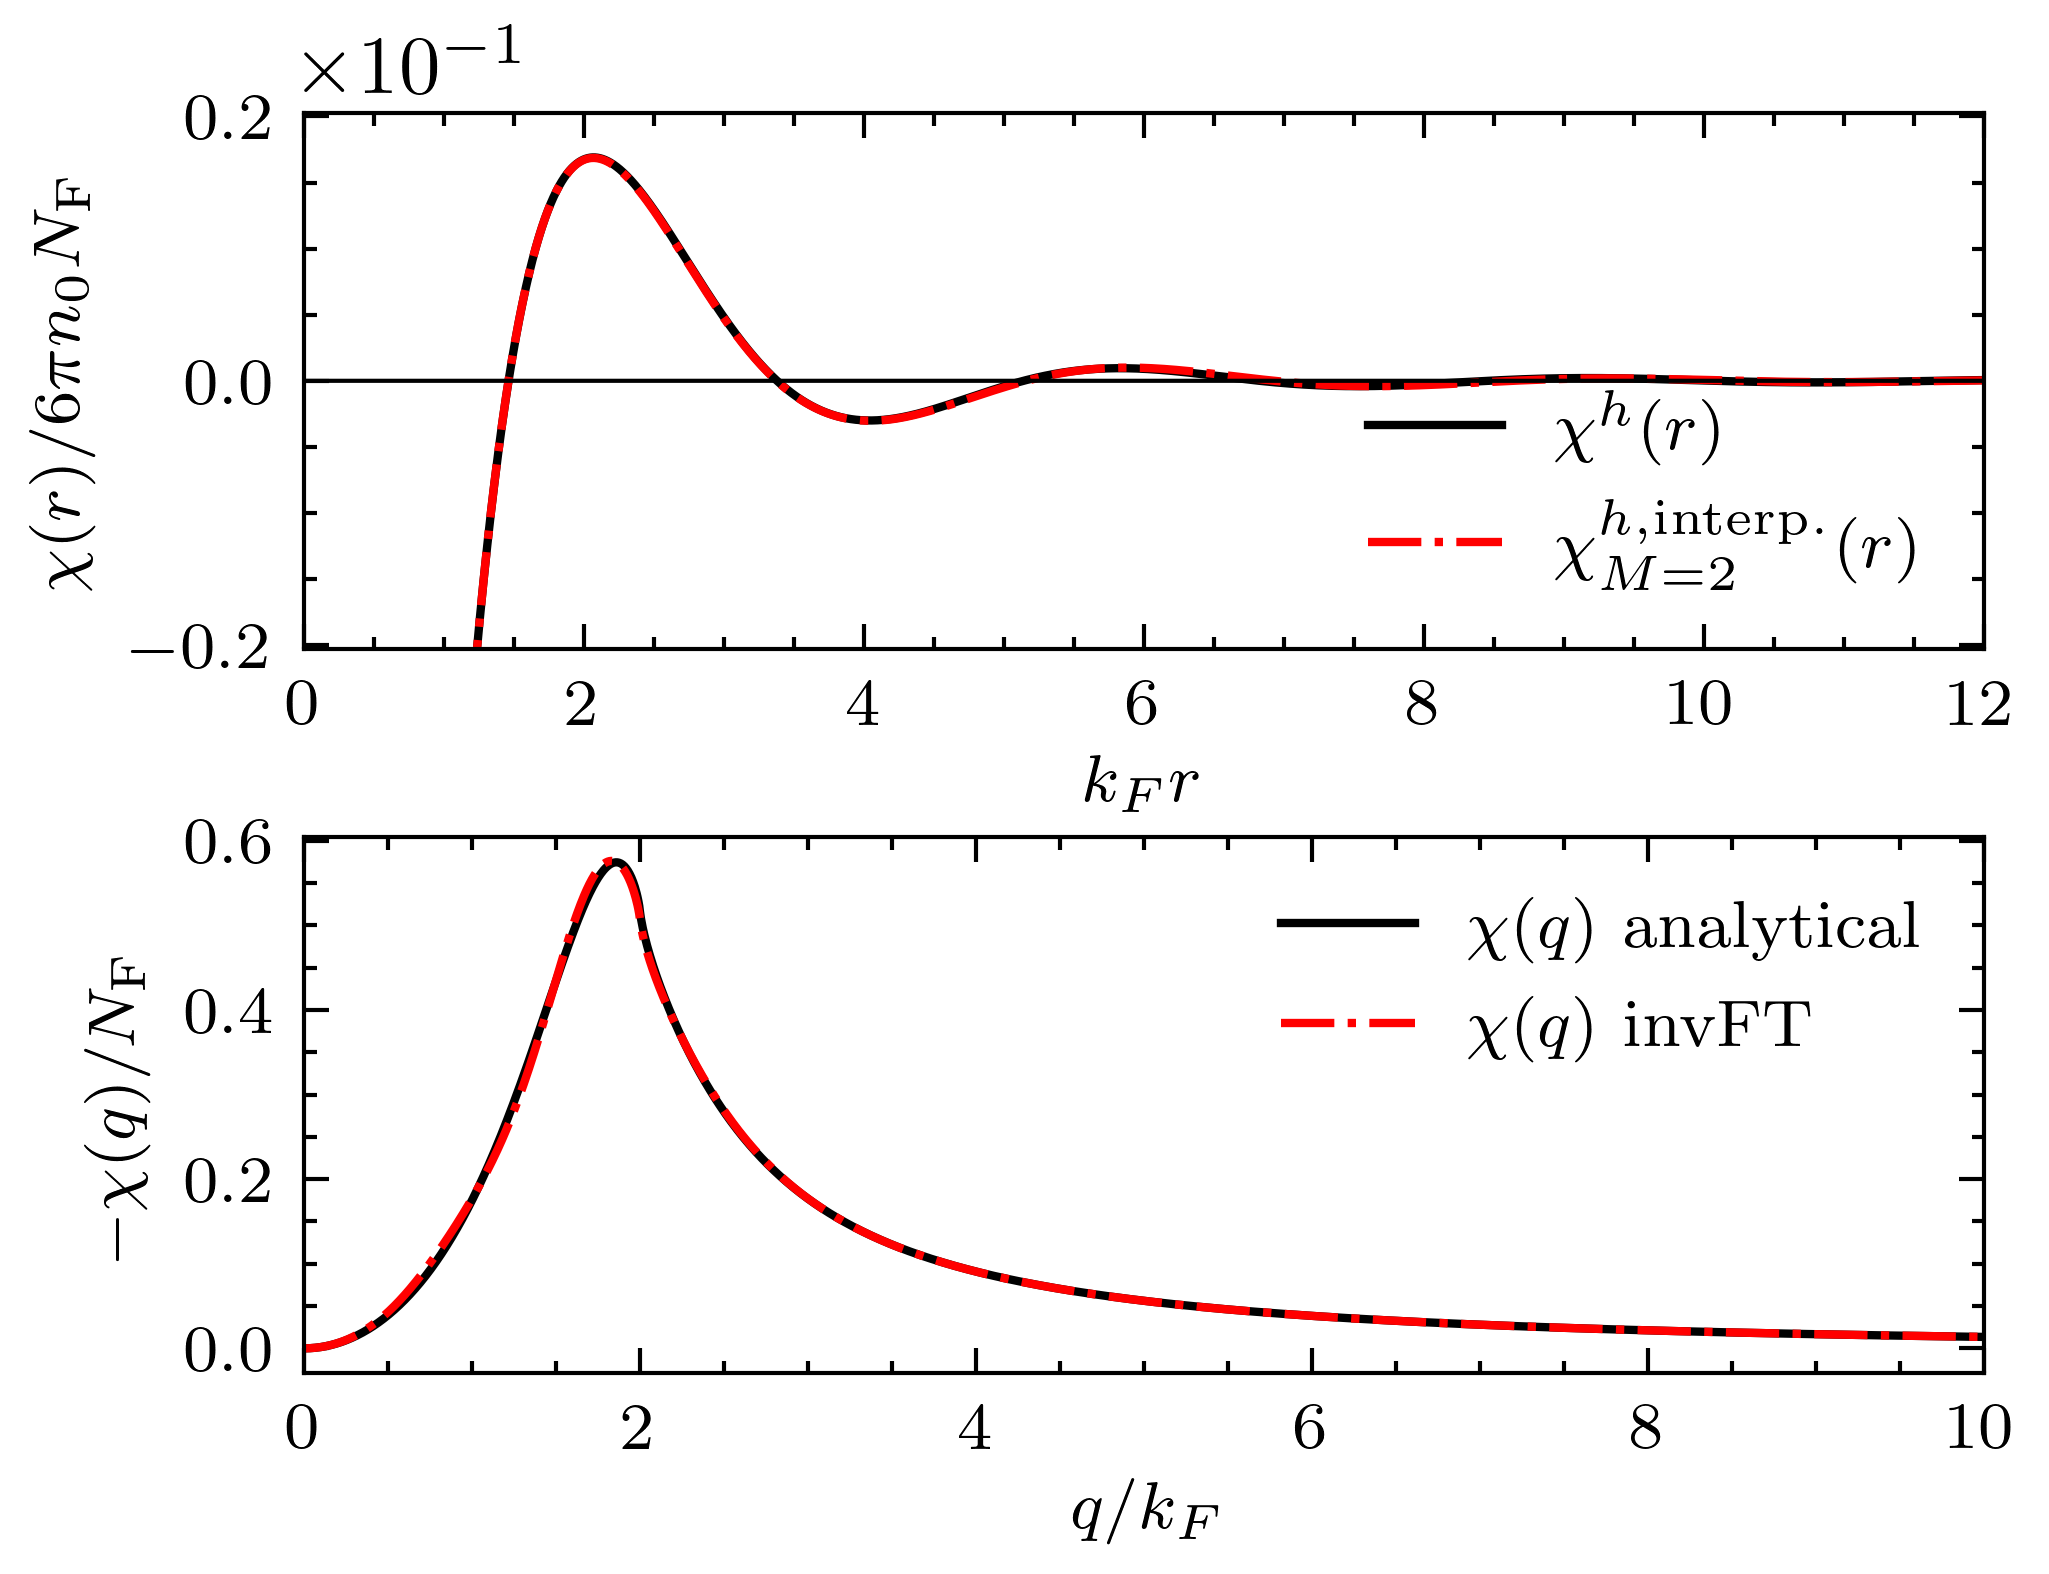
\includegraphics[width=0.46\textwidth]{Figs/delta_chi-rs10-error0.png}
    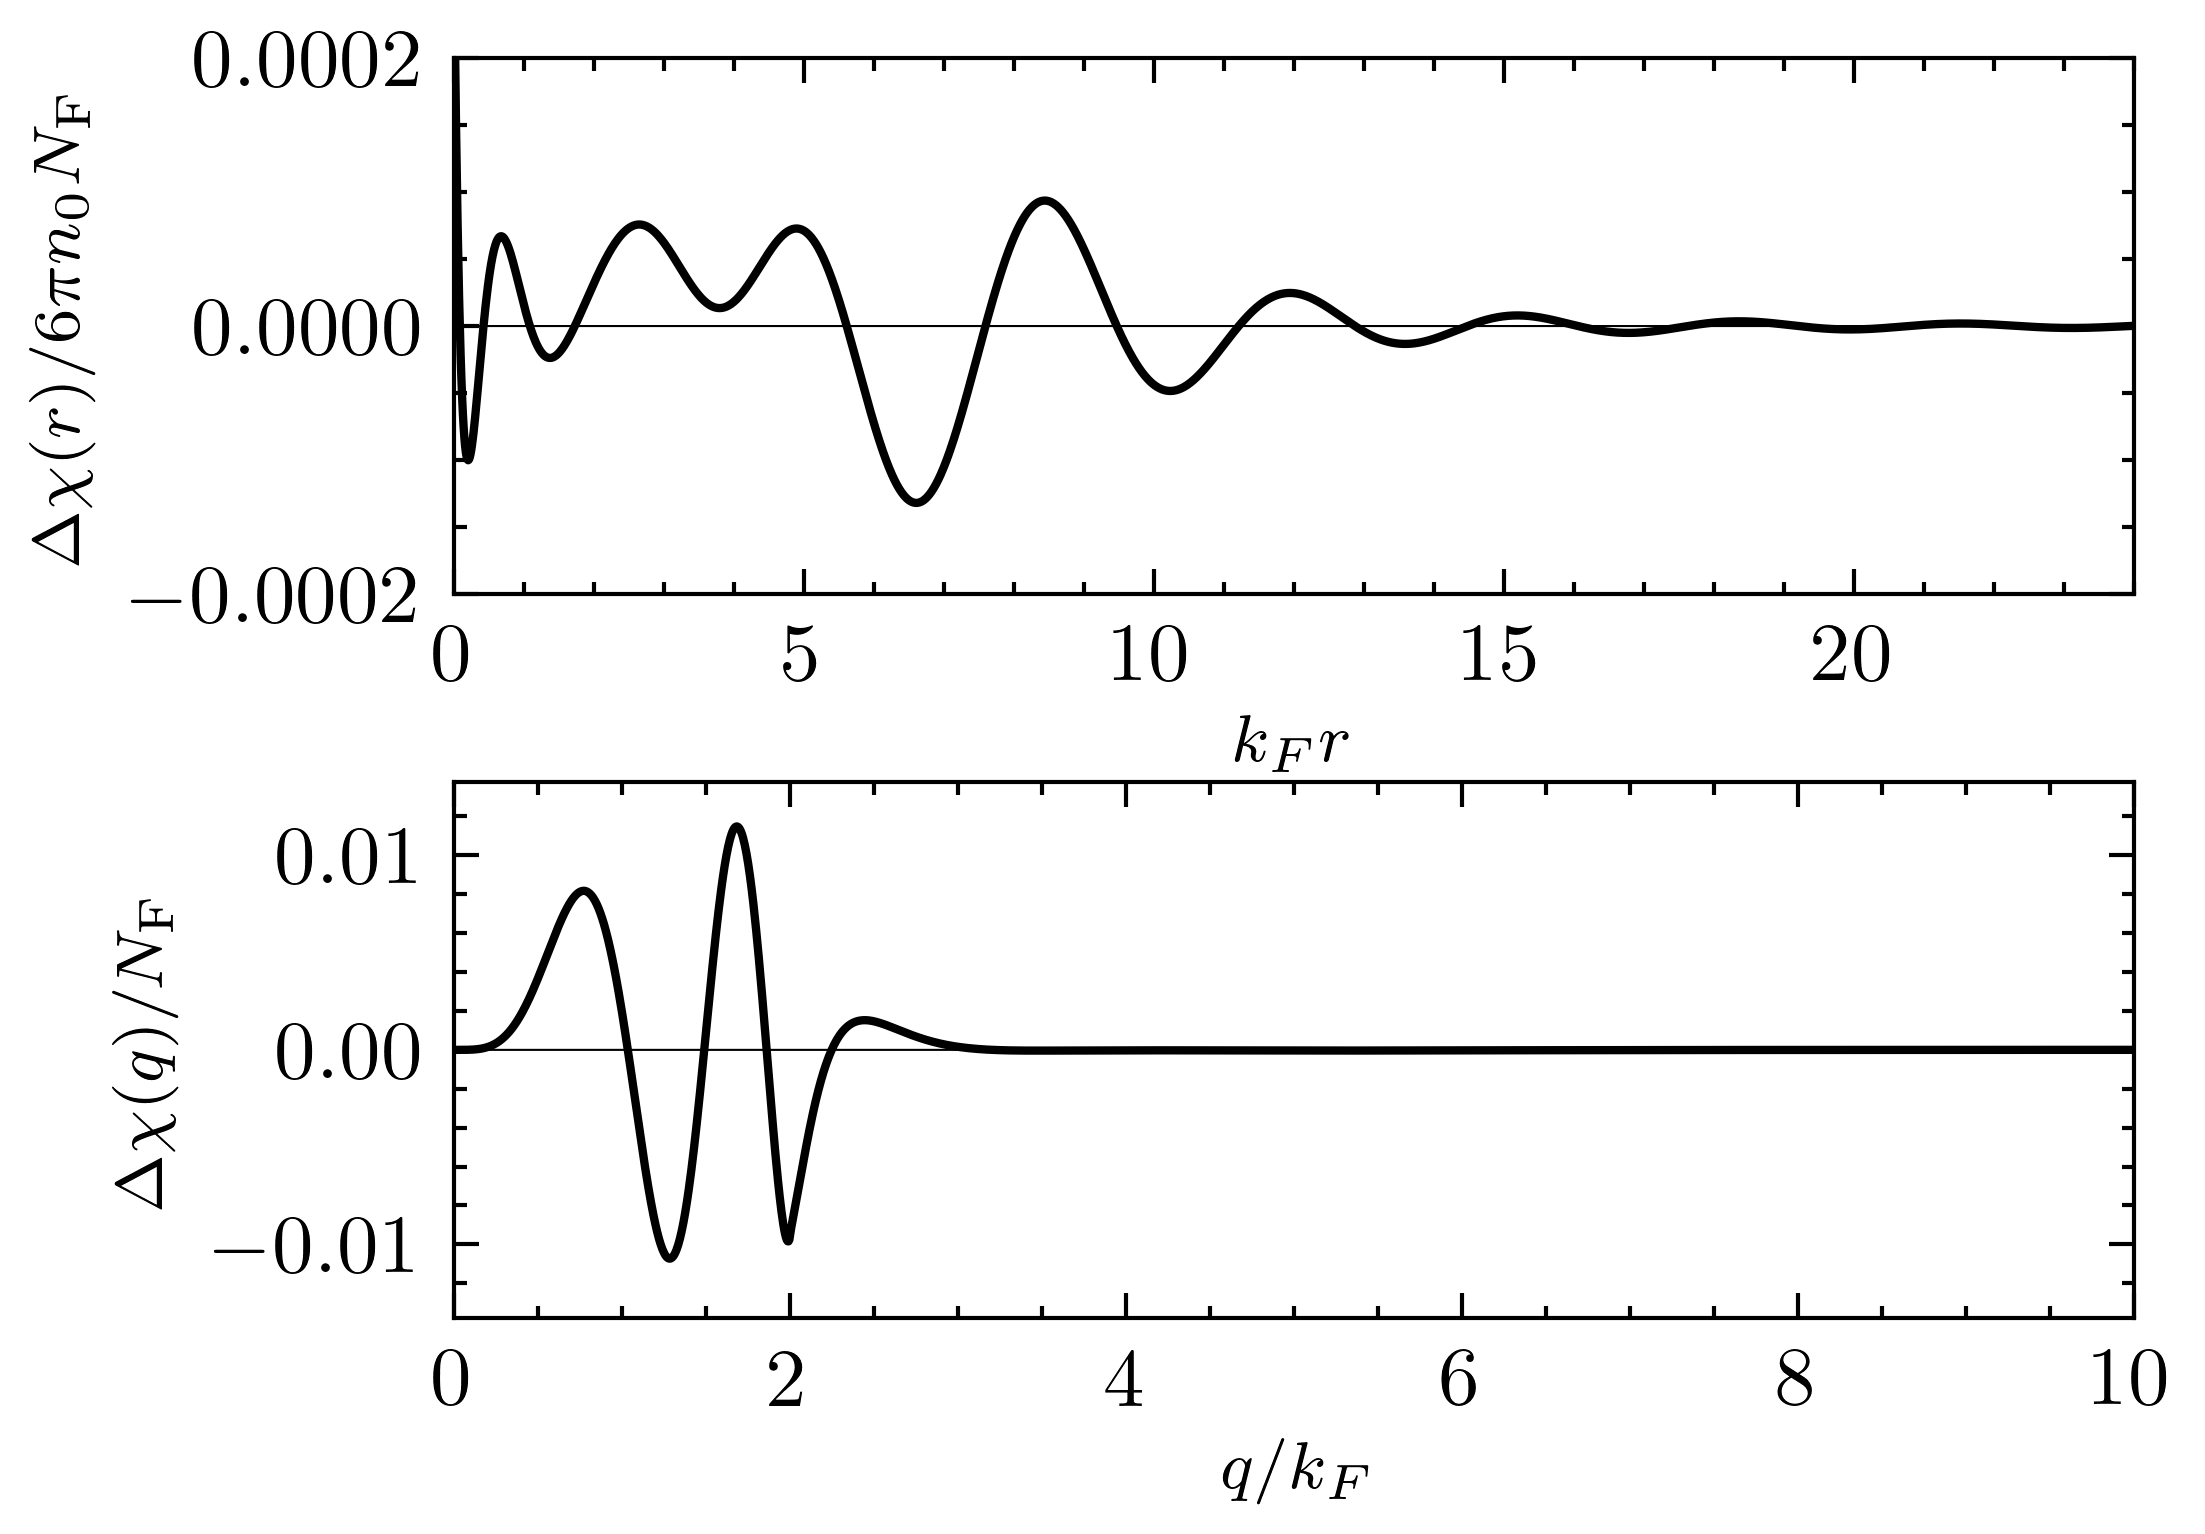
\includegraphics[width=0.49\textwidth]{Figs/delta_chi-rs10-error1.png}
    \caption{{\textbf{Left:}} Static response calculated by $\Delta{\chi}$-interpolation (in red) in comparison with the exact result (in black) for $r_s = 10$. {\textbf{Right:}} Normalized absolute error in static response calculated by $\Delta{\chi}$-interpolation. Upper panels show the real space quantities, and lower panel shows the reciprocal space quantities.}
    \label{fig:delta_chi-rs10}
\end{figure}

Since we eliminated the $r^{3-\gamma}$ factor when we defined $\Delta \chi$ in equation~\eqref{delta_chi_ansatz}, our optimizer is less constrained. This yields an even better performance around $k_Fr=0$  which leads to a quickly decaying error in large-$q$. These results are given in Figures \ref{fig:delta_chi-rs1} and \ref{fig:delta_chi-rs10}. It is important to note that when compared to Figure \ref{fig:qmc_differences}, all of our results are certainly within the margin of uncertainty of state-of-the art QMC methods.

\FloatBarrier
\subsection{$\{A_m, k_m,\alpha_m,\phi_m\}$ as a function of $r_s$}
Here, we observe the parameters $\{A_m, k_m,\alpha_m,\phi_m\}$ as a function of $r_s$. We see that in both interpolation cases, the parameters are very smooth (at least within this $r_s$ range) and quite easy to extract interpolations to be used for any $r_s$ this is the last step to complete the work.

\begin{figure}
    \centering
    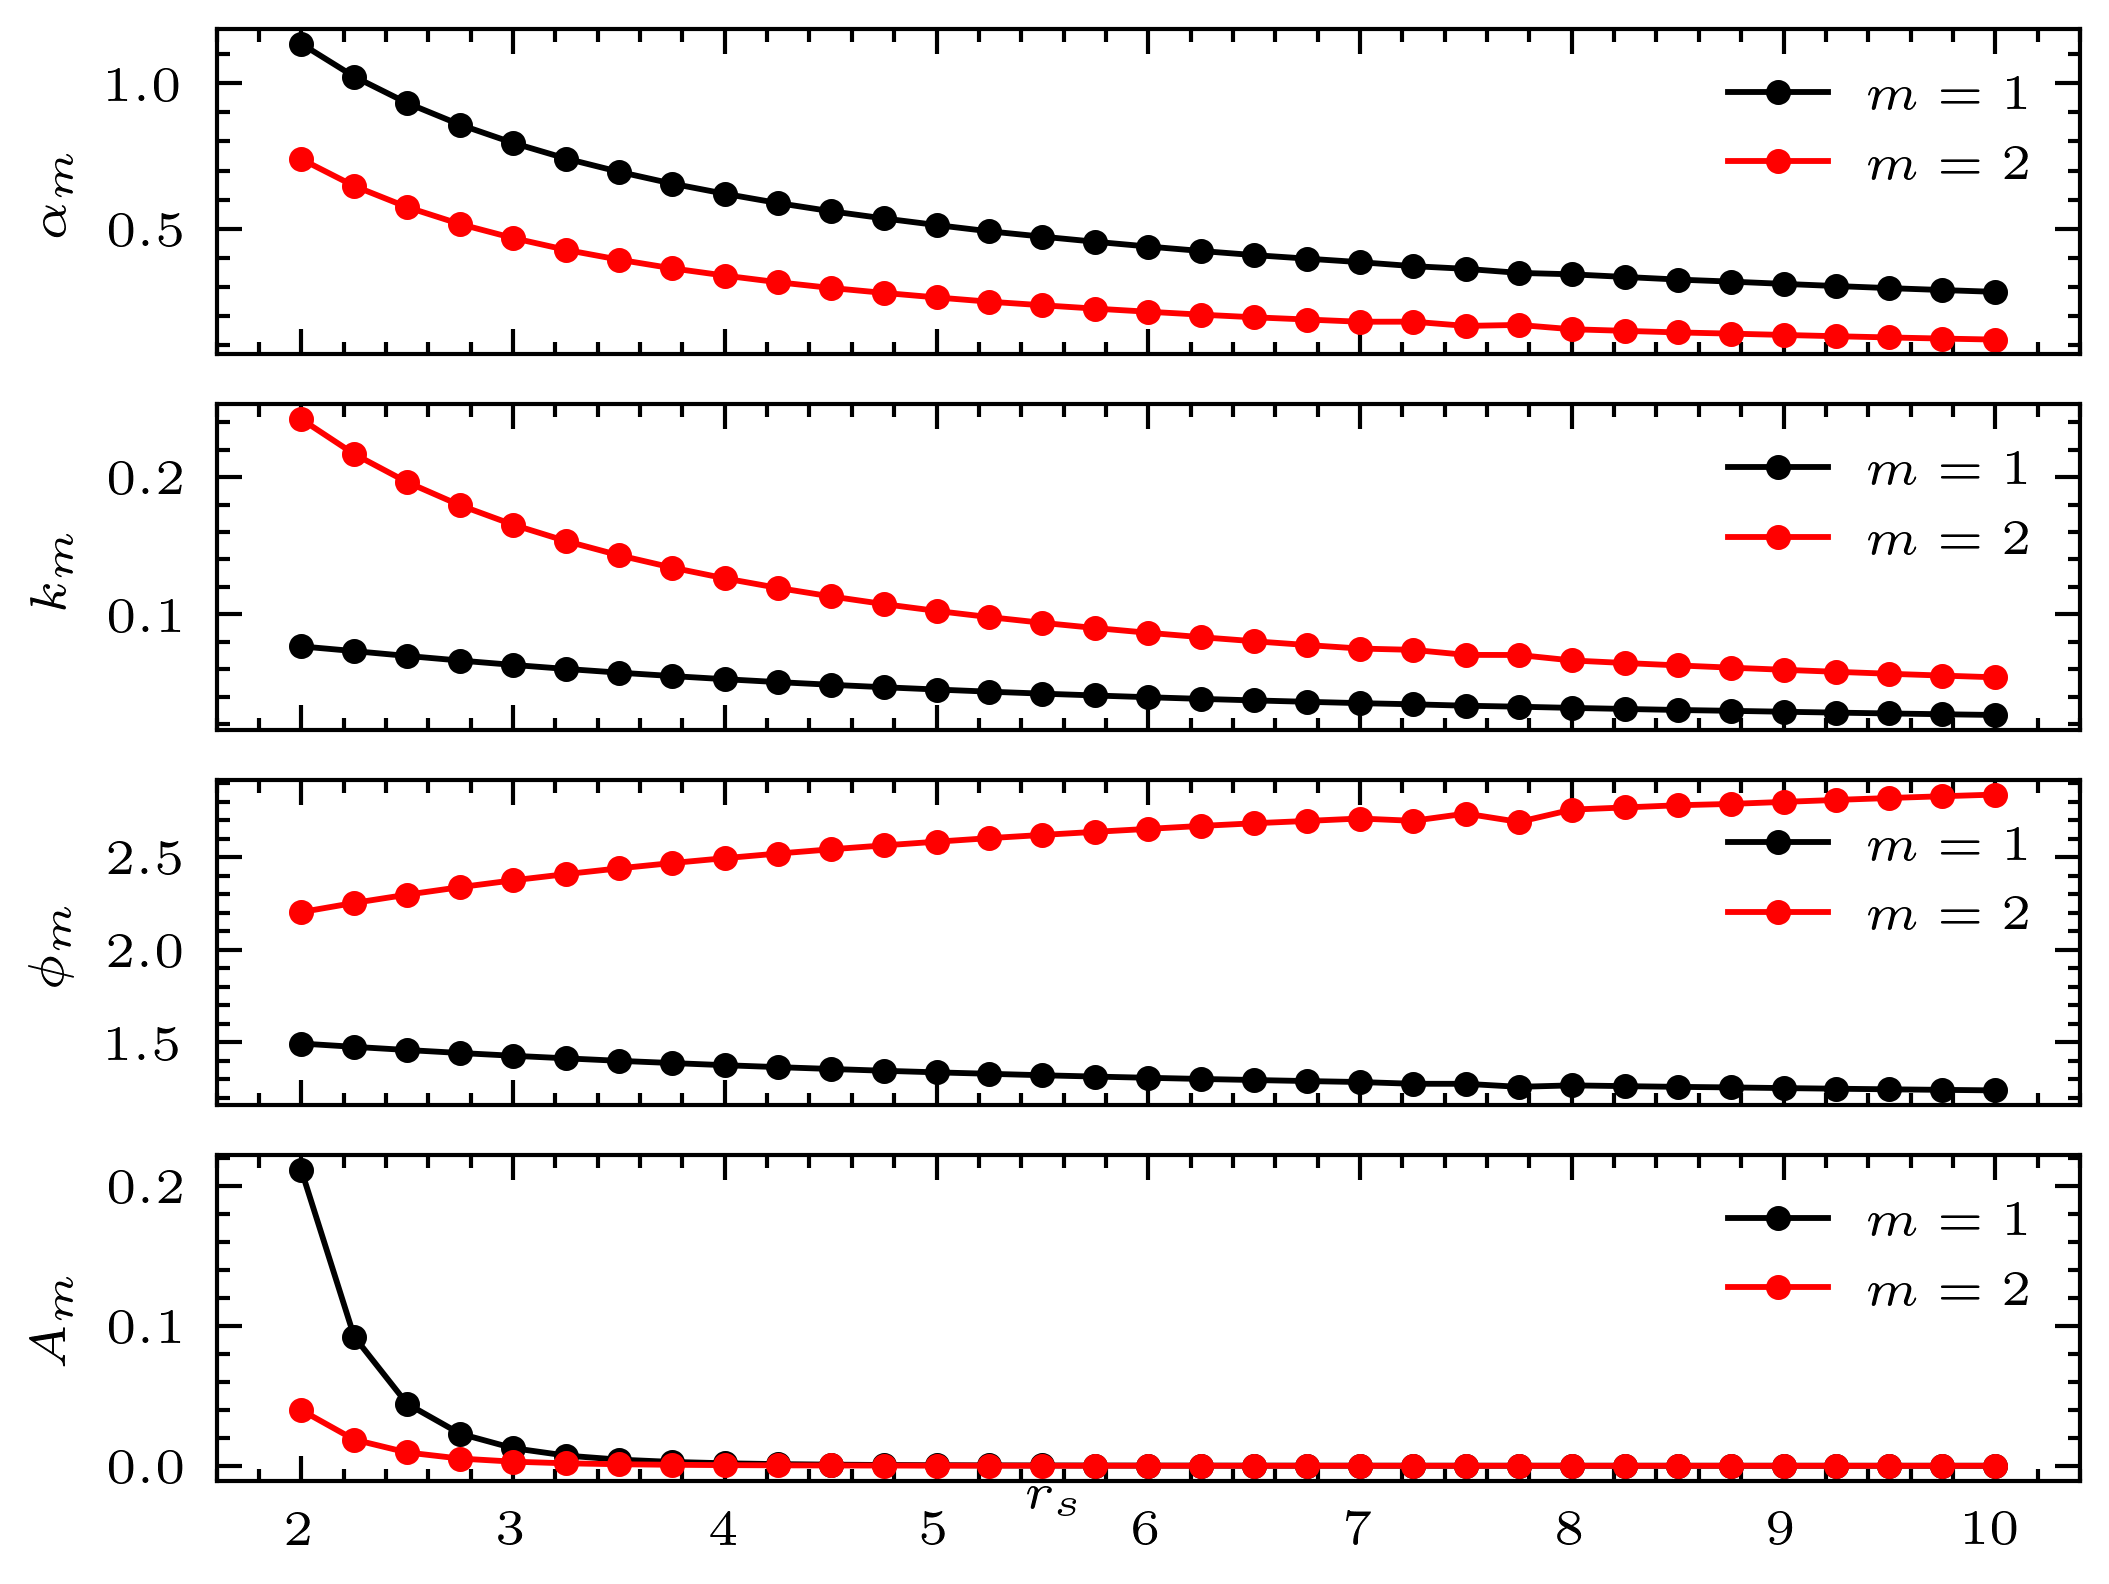
\includegraphics[width=0.6\textwidth]{Figs/parameters_X.png}
    \caption{Optimized parameters (first three plots) and exactly constrained $A_m$ (bottom panel) as a function of $r_s$, using $\mathcal{X}$-interpolation ($\gamma=2$).}
    \label{fig:parameters_X}
\end{figure}

\begin{figure}
    \centering
    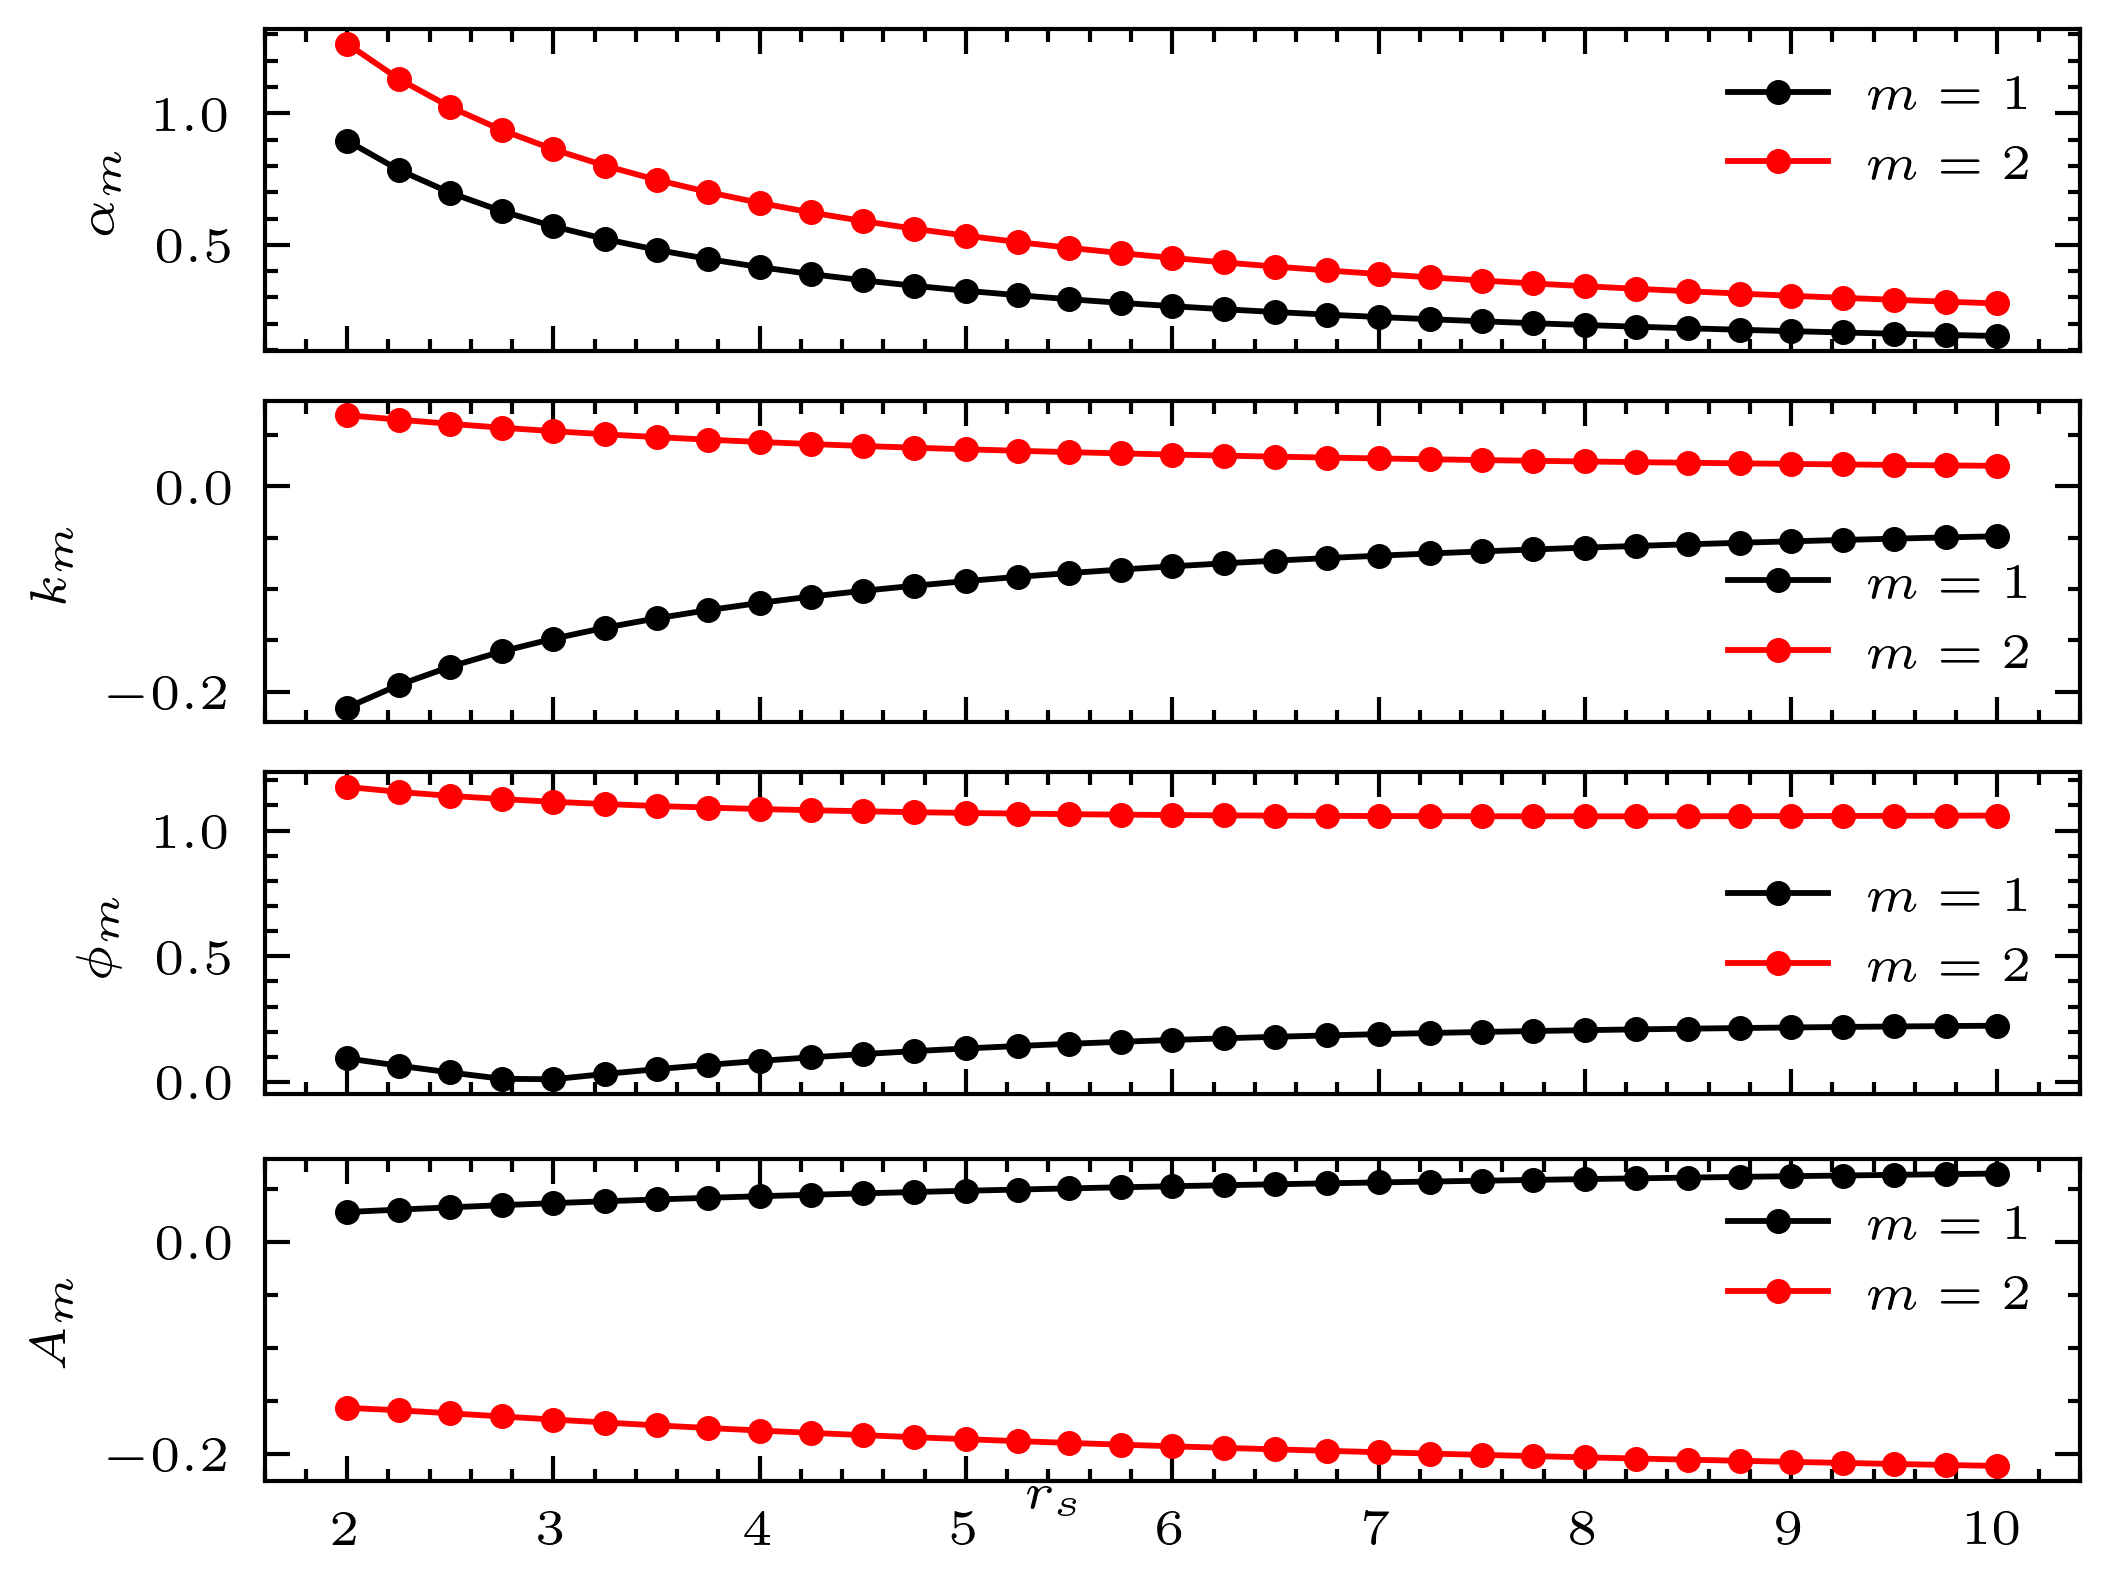
\includegraphics[width=0.6\textwidth]{Figs/parameters_delta-chi.png}
    \caption{Optimized parameters (first three plots) and exactly constrained $A_m$ (bottom panel) as a function of $r_s$, using $\Delta \chi$-interpolation.}
    \label{fig:parameters_delta_chi}
\end{figure}

\section{Preliminary connector results with interpolated $\chi(r)$}
Here, I show the effect of the interpolated-$\chi$ on the density within our method. Since we currently do not have the interpolation for full-$r_s$ range, I choose a single gas to calculate the linear response charge density, i.e.

\begin{equation}
    n(\mathbf{r};[v_\mathrm{ext}]) \simeq n^h(\bar v)    + \int \chi^h(\left| \mathbf{r} - \mathbf{r}' \right|, v^*_0 ) \left( v_\mathrm{ext}(\mathbf{r}') -  \bar v\right) d \mathbf{r}'
\end{equation}
where $\bar v$ is a value that fixes the number of electrons in the zeroth order, and $v^*_0$ corresponds to $r_s=2$ which is one of our optimized points.

\begin{figure}[h!]
    \centering
    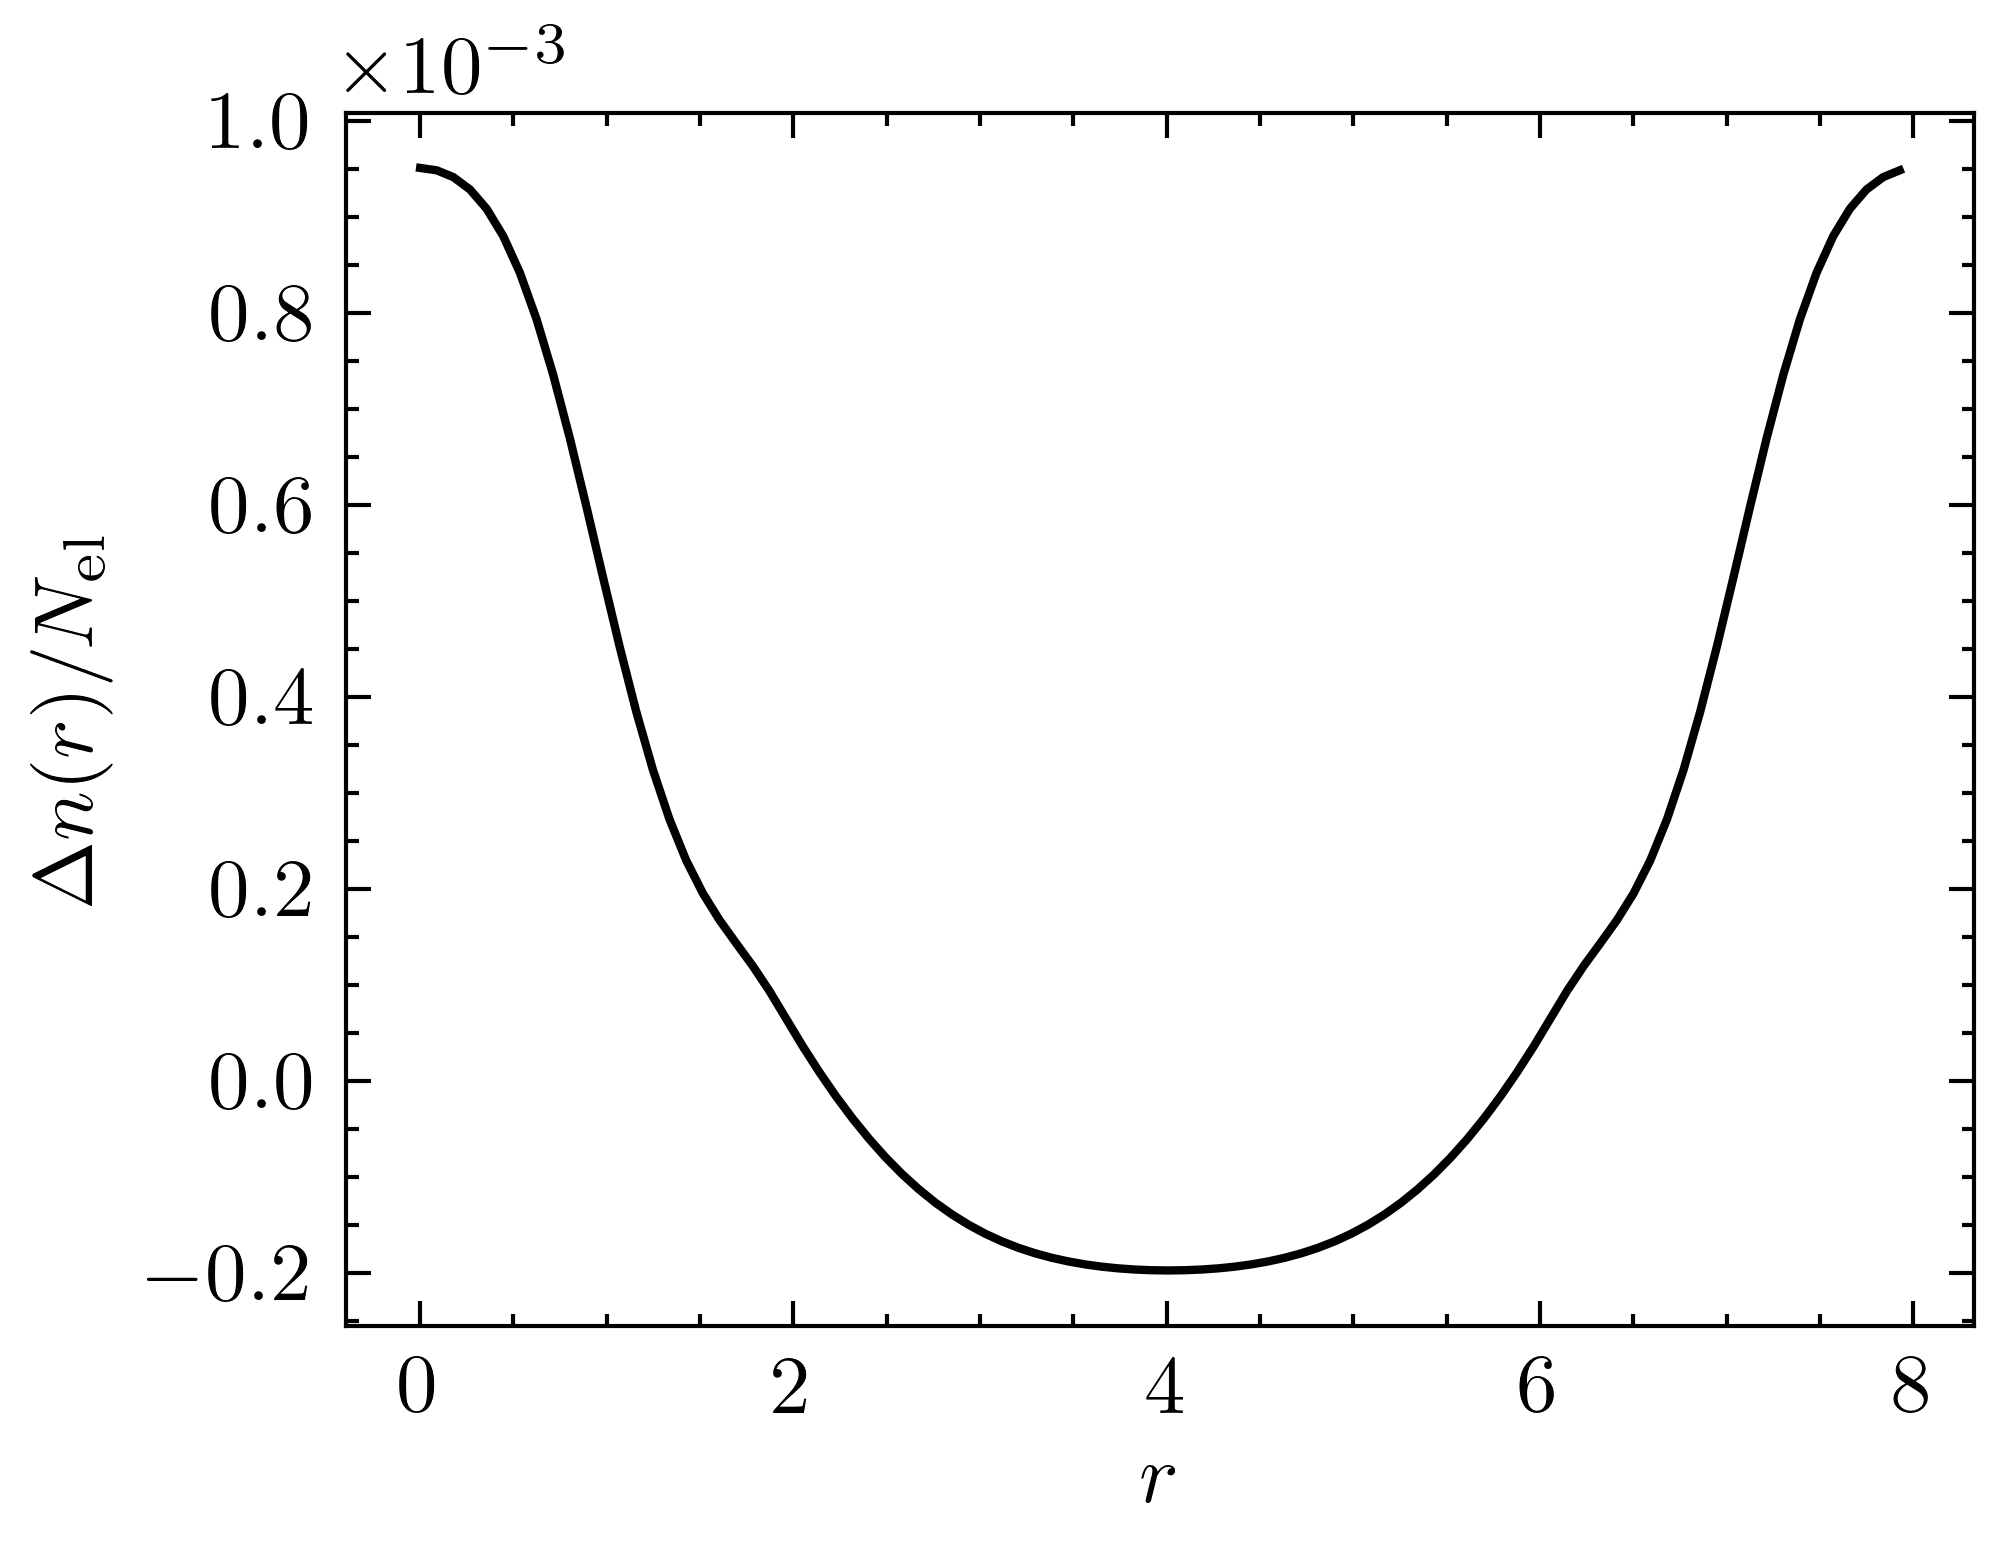
\includegraphics[width=0.6\textwidth]{Figs/delta_n.png}
    \caption{Charge density difference when used our previous procedure versus this work. The error is plotted in $100$ direction.}
    \label{fig:connector}
\end{figure}


Figure \ref{fig:connector} shows the density difference between when one uses inverse Fourier-transformed $\chi^h(q)$ (our previous procedure) and interpolated $\chi^h(r)$. As we can see, the normalized error is in the order of $10^{-4}$ which is really promising. Note that in this calculation, we chose a constant, single $v_0$. One needs to test the same after obtaining the full interpolation and check with $v_{0\mathbf{r}} = v_\mathrm{ext}(\mathbf{r})$.
\FloatBarrier
\bibliographystyle{apsrev4-2}
\bibliography{main}

\end{document}
